\newif\iffullversion
\fullversionfalse

\iffullversion
	\documentclass[11pt,letterpaper]{article}
	\usepackage[paper=letterpaper,margin=1in]{geometry}
\else
\documentclass[sigconf,anonymous]{acmart}
\settopmatter{printacmref=false} \settopmatter{printfolios=true}
\renewcommand\footnotetextcopyrightpermission[1]{} \pagestyle{plain} \fi 

\usepackage{amsmath,amsfonts,amssymb,tikz,multirow,stmaryrd,xspace,enumitem}
\usepackage{url}
\usepackage{amsthm}
\usepackage{caption}

\usepackage{amssymb}
\usepackage{pgfplots}
\pgfplotsset{compat=newest}

\usepackage{ellipsis, ragged2e, marginnote}

\usepackage[]{hyperref}

\hypersetup{
    colorlinks=true,
    linkcolor=darkred,
    citecolor=darkgreen,
    urlcolor=darkblue
}

\newcommand{\ytable}{\ensuremath{T}\xspace}
\newcommand{\Party}[1]{\ensuremath{P_{#1}}\xspace}

\newcommand{\false}{\ensuremath{\textsc{false}}\xspace}
\newcommand{\true}{\ensuremath{\textsc{true}}\xspace}

\newcommand{\naive}{na\"{\i}ve\xspace}
\newcommand{\Naive}{Na\"{\i}ve\xspace}

\newcommand{\share}[1]{\ensuremath{\llbracket #1\rrbracket}\xspace}
\newcommand{\shareA}[1]{\ensuremath{\llbracket #1\rrbracket}^{\textsf{A}}\xspace}
\newcommand{\shareTwo}[1]{\ensuremath{\llangle #1\rrangle}\xspace}

\newcommand{\Null}{\texttt{NULL}\xspace}
\newcommand{\XNull}{\ensuremath{X_\Null}\xspace}
\newcommand{\YNull}{\ensuremath{Y_\Null}\xspace}
\newcommand{\ZNull}{\ensuremath{Z_\Null}\xspace}

\newcommand{\F}{\ensuremath{\mathbb{F}}\xspace}
\renewcommand{\C}{\ensuremath{\mathcal{C}}\xspace}
\newcommand{\M}{\ensuremath{\mathcal{M}}\xspace}
\renewcommand{\O}{\ensuremath{\mathcal{O}}\xspace}
\renewcommand{\P}{\ensuremath{\mathcal{P}}\xspace}
\newcommand{\A}{\ensuremath{\mathcal{A}}\xspace}
\newcommand{\R}{\ensuremath{\mathcal{R}}\xspace}

\newcommand{\myvec}[1]{\boldsymbol{#1}}

\newcommand{\algorithm}[1]{\ensuremath{\text{\sf #1}}\xspace}

\newcommand{\DPFgen}{\algorithm{DPF.Gen}}
\newcommand{\DPFexpand}{\algorithm{DPF.Expand}}

\newcommand{\serv}[1]{server~\##1}
\newcommand{\Serv}[1]{Server~\##1}
\def\SSS{\ensuremath{\mathcal{S}}\xspace}
\def\RR{\ensuremath{\mathcal{R}}\xspace}
\newcommand{\Fpsi}[1]{\ensuremath{{\mathcal{F}^{#1}_{\textsf{psi}}}}\xspace}

\newcommand{\etal}{{\sl et~al.}\xspace}
\newcommand{\eg}{{\sl e.g.}\xspace}
\newcommand{\ie}{{\sl i.e.}\xspace}
\newcommand{\apriori}{{\sl a~priori\/}\xspace}


\newcommand{\rgets}{\overset{\$}\gets}

\newcommand{\command}[1]{\ensuremath{\text{\sc #1}}\xspace}

\newcommand{\subname}[1]{\ensuremath{\textsc{#1}}\xspace}
\newcommand{\mycmd}[1]{\textsc{#1}}

\newcommand{\codebox}[1]{\begin{varwidth}{\linewidth}\upshape \begin{tabbing}\quad\=\quad\=\quad\=\quad\=\kill
        #1
    \end{tabbing}\end{varwidth}}

\newcommand{\fcodebox}[1]{\framebox{\codebox{#1}}}






    \newtheorem{theorem}{Theorem}
    \newtheorem{definition}[theorem]{Definition}
    \newtheorem{claim}[theorem]{Claim}
\newtheorem{proposition}[theorem]{Proposition}


\newenvironment{proofof}[1]{\begin{proof}[Proof of #1.]}{\end{proof}}
\newenvironment{proofsketch}{\begin{proof}[Proof Sketch]}{\end{proof}}



\newcommand{\namedref}[2]{\hyperref[#2]{#1~\ref*{#2}}}
\newcommand{\stepref}[1]{\namedref{Step}{#1}}
\newcommand{\chapterref}[1]{\namedref{Chapter}{#1}}
\newcommand{\sectionref}[1]{\namedref{Section}{#1}}
\newcommand{\theoremref}[1]{\namedref{Theorem}{#1}}
\newcommand{\propositionref}[1]{\namedref{Proposition}{#1}}
\newcommand{\definitionref}[1]{\namedref{Definition}{#1}}
\newcommand{\corollaryref}[1]{\namedref{Corollary}{#1}}
\newcommand{\obsref}[1]{\namedref{Observation}{#1}}
\newcommand{\lemmaref}[1]{\namedref{Lemma}{#1}}
\newcommand{\claimref}[1]{\namedref{Claim}{#1}}
\newcommand{\figureref}[1]{\namedref{Figure}{#1}}
\newcommand{\tableref}[1]{\namedref{Table}{#1}}
\newcommand{\subfigureref}[2]{\hyperref[#1]{Figure~\ref*{#1}#2}}
\newcommand{\equationref}[1]{\namedref{Equation}{#1}}
\newcommand{\appendixref}[1]{\namedref{Appendix}{#1}}

\definecolor{darkred}{rgb}{0.5, 0, 0}
\definecolor{darkgreen}{rgb}{0, 0.5, 0}
\definecolor{darkblue}{rgb}{0, 0, 0.5}



\newcommand{\todo}[1]{\mbox{}\marginpar{\colorbox{red!80!black}{\textcolor{white}{to-do}}\vspace*{-22pt}}\textcolor{red}{#1}}

\renewcommand{\paragraph}[1]{\vspace{0.1cm}\noindent\emph{#1}.}
\newcommand{\myparagraph}[1]{\smallskip\noindent{\bf #1:}}
\newcommand{\DB}{\ensuremath{DB}\xspace}
\newcommand{\encode}[1]{\ensuremath{\llbracket #1 \rrbracket}}
\newcommand{\strLen}{e}
\newcommand{\f}[1]{\ensuremath{\mathcal{F}_{\textsc{#1}}}}
\newcommand{\proto}[1]{\ensuremath{\Pi_{\textsc{#1}}}}
\newcommand{\numbins}{\ensuremath{\beta}\xspace}
\newcommand{\cuckoobins}{\ensuremath{m}\xspace}
\newcommand{\binsize}{\ensuremath{\mu}\xspace}
\newcommand{\symsec}{\ensuremath{\kappa}\xspace}
\newcommand{\statsec}{\ensuremath{\lambda}\xspace}
\newcommand{\clientsetsize}{\ensuremath{n}\xspace}
\newcommand{\serversetsize}{\ensuremath{N}\xspace}
\newcommand{\elsize}{\ensuremath{\rho}\xspace}
\newcommand{\binScale}{\ensuremath{c}\xspace}
\newcommand{\pirblocksize}{\ensuremath{b}\xspace}
\newcommand{\cuckooexpansion}{\ensuremath{e}\xspace}
\newcommand{\cuckootable}{\ensuremath{CT}\xspace}





\makeatletter
\DeclareFontFamily{OMX}{MnSymbolE}{}
\DeclareSymbolFont{MnLargeSymbols}{OMX}{MnSymbolE}{m}{n}
\SetSymbolFont{MnLargeSymbols}{bold}{OMX}{MnSymbolE}{b}{n}
\DeclareFontShape{OMX}{MnSymbolE}{m}{n}{
	<-6>  MnSymbolE5
	<6-7>  MnSymbolE6
	<7-8>  MnSymbolE7
	<8-9>  MnSymbolE8
	<9-10> MnSymbolE9
	<10-12> MnSymbolE10
	<12->   MnSymbolE12
}{}
\DeclareFontShape{OMX}{MnSymbolE}{b}{n}{
	<-6>  MnSymbolE-Bold5
	<6-7>  MnSymbolE-Bold6
	<7-8>  MnSymbolE-Bold7
	<8-9>  MnSymbolE-Bold8
	<9-10> MnSymbolE-Bold9
	<10-12> MnSymbolE-Bold10
	<12->   MnSymbolE-Bold12
}{}

\let\llangle\@undefined
\let\rrangle\@undefined
\DeclareMathDelimiter{\llangle}{\mathopen}{MnLargeSymbols}{'164}{MnLargeSymbols}{'164}
\DeclareMathDelimiter{\rrangle}{\mathclose}{MnLargeSymbols}{'171}{MnLargeSymbols}{'171}
\makeatother


 
\begin{document}





\title{Fast Database Joins and PSI for Secret Shared Data}
\begin{abstract}
We present a scalable protocol for database joins on secret shared data in the honest-majority three-party setting. The key features of our protocol are a rich set of SQL-like join/select queries and the ability to compose join operations together due to the inputs and outputs being generically secret shared between the parties. Provided that all joins operate on unique primary keys, no information is revealed to any party during the protocol. In particular, not even the sizes of intermediate joins are revealed. All of our protocols are constant-round and achieve $O(n)$ communication and computation overhead for joining two tables of $n$ rows. 

These properties make our protocol ideal for \emph{outsourced secure computation}. In this setting several non-colluding servers are setup and the input data is shared among them. These servers then perform the relevant secret shared computation and output the result. This model has recently been gaining traction in industry, e.g. Facebook's Crypten, Cape Privacy's TFEncrypted, Mozilla Telemetry.

We additionally implement two applications on top of our framework. The first application detects voter registration errors within and between agencies of 50 US states, in a privacy-preserving manner. The second application allows several organizations to compare network security logs to more accurately identify common security threats, e.g. the IP addresses of a bot net. In both cases, the practicality of these applications depends on efficiently performing joins on millions of secret shared records. For example, our three party protocol can perform a join on two sets of 1 million records in 4.9 seconds or, alternatively, compute the cardinality of this join in just 3.1 seconds. 
\end{abstract}

\iffullversion
\else
\maketitle
\fi

\section{Introduction}

We consider the problem of performing SQL-style join operations on tables that are secret shared among three parties, in the presence of an honest majority. Our proposed protocol takes two or more arbitrarily secret shared database tables and constructs another secret shared table containing a \texttt{join} of the two tables, without revealing \emph{any} information beyond the secret shares themselves. Our protocol is constant-round and  has computation and communication overhead that is linear in the size of the tables. Simulation-based security is achieved in the semi-honest setting with an honest-majority. Our protocol can perform inner, left and full joins along with union and arbitrary computation on the resulting table, with the best performance and security guarantees when joins operate on unique primary keys.

New techniques \cite{usenix:PSZ14,USENIX:PSSZ15,PSZ16,CCS:KKRT16,PSWW18,CLR17,CHLR18,cryptoeprint:2017:738,RA17,KLSAP17,OOS17,KMPRT17} for performing set intersection, inner join and related functionalities have shown great promise for practical deployment. 
The vast majority of these works perform {\em private set intersection} (PSI), which is analogous to revealing the entire result of an inner join.
Computing a join {\em without revealing it} (\ie, performing further joins, filtering, or computing only aggregate information) is significantly harder, and optimizations for such a setting do not automatically translate to our composable setting.
We highlight a few notable results that hide the contents of a join (revealing only some function of it):

Ion et al.\ recently deployed a private set intersection sum protocol\cite{cryptoeprint:2017:738} to allow customers of Google Adwords to correlate online advertising with offline sales, while preserving user privacy. Pinkas et al. \cite{PSWW18} also introduced a practical protocol that can compute any (symmetric) function of the intersection and associated data. These protocols can be framed in terms of SQL queries consisting of an inner join followed by an aggregation on the resulting table, e.g. summing a column.  
Neither of these protocols (and almost no prior related results) support secret-shared inputs, but rather require the source tables to be held in the clear by each party.

The majority of these protocols consider the two party setting and are based on various cryptographic primitives, e.g. exponentiation~\cite{cryptoeprint:2017:738}, oblivious transfer\cite{PSWW18}, or fully homomorphic encryption\cite{CLR17}. However, in this work we alter the security model to consider three parties with an honest majority. The motivation is that typical protocols in this setting (e.g.\cite{highthroughput}) require less computation and communication than similar two party protocols, by a factor of at least the security parameter $\kappa=128$. Moreover, we will see that the honest majority enables various algorithms which are orders of magnitude more efficient, e.g. oblivious permutations require $O(n)$ work instead of $O(n\log n \kappa)$ \cite{MS13}. 

Given this observation we investigate how to leverage the efficiency gains in the three party setting to construct practical protocols for performing set intersection and other SQL-like operations where both the inputs and outputs are secret shared. One critical aspect of this input/output requirement is that join operations can then be \emph{composed} together, where the output of a join can be the input to another. Allowing this composability greatly increases the ability to perform highly complex queries and enables external parties to contribute data simply by secret sharing it between the primary parties which participate in the protocol.

The fact that we support secret-shared inputs also leads to \emph{outsourced secure computation.} Three non-coluding servers can be established, and inputs can be provided by the servers themselves or by external parties simply by secret sharing the input among the servers. This model has been gaining traction in industry. Mozilla recently deployed a service to collect telemetry data about Firefox\cite{mozilla} using two non-colluding servers running the Prio protocol\cite{DBLP:conf/nsdi/Corrigan-GibbsB17}. Other examples include privacy preserving machine learning frameworks which support secret shared inputs such as Facebook's Crypten built for PyTorch\cite{Crypten} and Cape Privacy's FTEncrypted built for TensorFlow\cite{TFEncrypted}. 

Complex joins on secret-shared inputs/outputs are valuable in all of these examples.
Most privacy preserving machine learning publications\cite{aby3,Crypten,TFEncrypted,SecureNN,XONN} assume that the data being trained on has already been joined together. However, without a framework like ours it is unclear how this would be accomplished while preserving privacy and efficiency. The generality of our approach allows us to solve these problems and many others, e.g. the two applications presented in \sectionref{sec:app}.


\subsection{Functionality}

Our protocol offers a wide variety of functionality including set intersection, set union, set difference and a variety of SQL-like joins with complex boolean queries. Generally speaking, our protocol works on tables of secret shared data which are functionally similar to SQL tables. This is in contrast to traditional PSI and PSU protocols\cite{usenix:PSZ14,USENIX:PSSZ15,PSZ16,CCS:KKRT16} in that each record is now a tuple of values as opposed to a single key. 

We define our database tables in the natural way. Each table can be viewed as a collection of rows or as a vector of columns. For a table $X$, we denote the $i$th row as $X[i]$ and the $j$th column as $X_j$. 
\iffullversion
Note that each column of a table has the same length but can contain different data types, e.g. $X_1$ is a column of 32 bit fixed point decimal values and $X_2$ is a column of 1024 bit strings.

\fi
Our core protocol requires each table to contain unique values in the column defining the join  (i.e., we can only join on ``unique primary keys''). For example, if we consider the following SQL styled join/intersection query
\vspace{-0.1cm}
$$
\texttt{select } X_2 \texttt{ from } X \texttt{ inner join } Y \texttt{ on } X_1 = Y_1
\vspace{-0.1cm}
$$
then the join-keys are $X_1$ and $Y_1$. This uniqueness condition can be extended to the setting where multiple columns are being compared for equality. 
\iffullversion
In this case the tuple of these columns must be unique. 
\fi
Later on we will discuss the case when such a uniqueness property does not hold. Our protocols also support a \texttt{where} clause that filters the selection using an arbitrary predicate of the $X$ and $Y$ rows. Furthermore, the \texttt{select} clause can also return a function of the two rows. For example,
\vspace{-0.1cm}
\begin{align*}
\texttt{select }&  X_1,max(X_2, Y_2)  \texttt{ from } X \texttt{ inner join } Y \\
\texttt{on }& X_1 = Y_1 \texttt{ where } Y_2 > 23.3
\vspace{-0.1cm}
\end{align*}
In general, the supported join operations can be characterized in three parts: 1) The select function $S(\cdot)$ that defines how the rows of $X,Y$ are used to construct each output row, e.g. $S(X,Y)=(X_1, max(X_2,Y_2))$
\iffullversion
in the example above
\fi. 2) The predicate $P(\cdot)$ that defines the \texttt{where} clause, and 3) which columns are being joined on.
\iffullversion
 We require that both $S$ and $P$ must be expressible in the framework of \cite{aby3} which we provide a custom implementation of.
\fi

\iffullversion
So far we have discussed inner join (intersection) between two tables. 
\fi
Several other types of joins are also supported including left and right joins, set union and set minus (difference) and full joins. A left join takes the inner join and includes all of the missing records from the left table. For the records solely from the left table, the resulting table contains \texttt{NULL} for the columns from the right table. Right join is defined symmetrically. A full join is a natural extension where all the missing rows from $X$ and $Y$ are added to the output table.

We define the union of two tables to contain all records from the left table, along with all the records from the right table which are not in the intersection with respect to the join-keys. Note that this definition is not strictly symmetric with respect to the left and right tables due to rows in the intersection coming from the left table. Table minus is similarly defined as all of the left table whose join-column value is not present in the right table. 

Beyond these various join operations, our framework supports two broad classes of operations which are a function of a single table. The first is a general SQL select statement which can perform computation on each row (e.g. compute the max of two columns) and filter the results using a \texttt{where} clause predicate. The second class is referred to as an aggregation which performs an operation across all of the rows of a table --- for example, computing the sum, counts, or the max of a given column. 
\subsection{Our Results}

We present the first practical secure multi-party computation protocol for performing SQL-style database joins with linear overhead and constant rounds. Our protocol is fully composable in that the input and output tables are generically secret shared between the parties. 
\iffullversion
	No partial information is revealed at any point. 
\fi
	We achieve this result by combining various techniques from private set intersection and secure computation more 
\iffullversion 
	broadly while requiring the joined on keys be unique.
\else
	broadly.
\fi
 We build on the the binary secret sharing technique of \cite{highthroughput} with enhancements described by \cite{aby3}. We then combine this secret sharing scheme with cuckoo hashing\cite{usenix:PSZ14}, an MPC friendly PRF\cite{lowmc} and a custom protocol for evaluating an oblivious switching network\cite{MS13}. Using these building blocks our protocol is capable of computing the intersection of two tables of $n=2^{20}$ rows in 4.9 seconds. 
\iffullversion 
	Alternatively, the cardinality of the intersection can be computed in just 3.1 seconds.
\fi
  Beyond these two specific functionalities, our protocol allows arbitrary computation applied to a shared table. Compared to existing three party protocols with similar functionality (composable), our implementation is roughly $1000\times$ faster. When compared with \emph{non-composable} two party protocol, we observe a larger difference ranging from our protocol being $1.25\times$ slower to $4000\times$ faster depending on the functionality. 


Building on our proposed protocol we demonstrate its utility by showcasing two potential applications. The first prototype would involve running our protocol between and within the states of the United States to validate the accuracy of the voter registration data in a privacy preserving way. The Pew Charitable Trust\cite{pew} reported 1 in 8 voter registration records in the United States contains a serious error while 1 in 4 eligible citizens remain unregistered. Our privacy preserving protocol identifies when an individual's address is out of date or more seriously if someone is registered to vote in more than one state which could allow them to cast two votes. 
\iffullversion
Additionally, our protocol can help register eligible citizens. Our protocol ensures that only the minimum amount of information is revealed, namely the identities of individuals with serious registration errors.
\fi 
Due to how the data is distributed between different governmental agencies, it will be critical that our protocol allows for composable operations. We implement this application and demonstrate that it is practical to run at a national scale (250M records) and low cost.

The second application that we consider allows multiple organizations to compare computer security incidents and logs to more accurately identify unwanted activities, e.g. a bot net. Several companies already offer this service including Facebook's ThreatExchange\cite{threat} and an open source alternative\cite{alt_threat}. One of the primary limitations of these existing solutions is the requirement that each organization send their security logs to a central party, e.g. Facebook. We propose using our protocol to distribute the trust of this central party between three parties such that privacy is guaranteed so long as there is an honest majority.


\subsection{Related Work}
We now review several related works that use secure computation techniques. With respect to functionality the closest related work is that of Blanton and Aguiar\cite{ASIACCS:BlaAgu12} which describes a relatively complete set of protocols for performing intersections, unions, set difference, etc. and the corresponding SQL-like operations. Moreover, these operations are composable in that the inputs and outputs are secret shared between the parties. At the core of their technique is the use of a generic MPC protocol and an oblivious sorting algorithm that merges the two sets. This is followed by a linear pass over the sorted data where a relation is performed on adjacent items. Their technique has the advantage of being very general. However, the proposed algorithm has complexity $O(n \log^2 n)$, is not constant round\footnote{It is not constant round when the underlying MPC protocol is not constant round which is typically required for high throughput.},  and also requires unique join keys. 
\iffullversion
As a result, the implementation from 2011 performed poorly by current standards, intersecting $2^{10}$ items in 12 seconds. The modern protocol \cite{CCS:KKRT16} which is \emph{not composable} can perform intersections of $2^{20}$ items in 4 seconds. While this difference of three orders of magnitude would narrow if reimplemented using modern techniques, the gap would remain large.
\else
This results in poor concrete performance as shown in \sectionref{sec:eval}.
\fi


\iffullversion
Huang, Evans and Katz\cite{HEK12} also described a set intersection protocol based on sorting. Unlike \cite{ASIACCS:BlaAgu12}, this work considers the two party setting where each party holds a set in the clear.
This requirement prevents the protocol from being composable but allows the complexity to be reduced to $O(n\log n)$. The key idea is that each party locally sorts their set followed by merging the sets within MPC. The protocol can then perform a single pass over the sorted data to construct the intersection. While this results in performance improvements the overall protocol requires  $O(n\log n)$ operations and is not composable.
\fi

\iffullversion
Another line of work was begun by Kissner and Song\cite{KS06} and improved on by \cite{MF06}. Their approach is based on the observation that set intersection and multi-set union have a correspondence to operations on polynomials. A set $S$ can be encoded as the polynomial $\hat S(x)= \prod_{s\in S}(x-s)\in \mathbb{F}[x]$. That is, the polynomial $\hat S(x)$ has a root at all $s\in S$. Given two such polynomials, $\hat S(x), \hat T(x)$, the polynomial encoding the intersection is $\hat S(x)+\hat T(x)$ with overwhelming probability given a sufficiently large field $\mathbb{F}$.

Multi-set union can similarly be performed by multiplying the two polynomials together. Unlike with normal union, if an item $y$ is contained in $S$ and $T$ then $\hat S(x)\hat T(x)$ will contain two roots at $y$ which is often not the desired functionality. This general idea can be transformed into a secure multi-party protocol using oblivious polynomial evaluation\cite{NP99} along with randomizing the result polynomial. The original computational overhead was $O(n^2)$ which can be reduced to the cost of polynomial interpolation $O(n\log n)$ using techniques from \cite{MF06}. The communication complexity is linear. In addition, this scheme assumes an ideal functionality to generate a shared Paillier key pair. We are unaware of any efficient protocol to realize this functionality except for \cite{RSA:HMRT12} in the two party setting.

This general approach is also composable. However, due to randomization that is performed the degree of the polynomial after each operation doubles. This limits the practical ability of the protocol to compose more than a few operations. Moreover, it is not clear how this protocol can be extended to support SQL-like queries where elements are key-value tuples. This general approach is also composable but incurs a 2 times overhead for each successive operations and cannot be extended to SQL-like queries. 
\fi


\iffullversion
Hazay and Nissim\cite{HN12} introduce a pair of protocols computing set intersection and union which are also based on oblivious polynomial evaluation where the roots of the polynomial encode a set. However, these protocols are restricted to the two party case and are not composable. The non-composability comes from the fact that only one party constructs a polynomial $\hat S(x)$ encoding their set $S$ while the other party obliviously evaluates it on each element in their set. The result of these evaluations are compared with zero\footnote{The real protocol is slightly more complicated than this.}. These protocols have linear overhead and can achieve security in the malicious setting.
\fi

Pinkas, Schneider and Zohner \cite{usenix:PSZ14} introduced a paradigm for set intersection that combines a hash table technique known as cuckoo hashing with a randomized encoding technique using oblivious transfer. Due to the hashing technique, the problem is reduced to comparing a single item $x$ to a small set $\{y_1,...,y_m\}$. Oblivious transfer is then used to interactively compute the randomized encoding $x'$ of $x$ while the other party locally computes the encodings $\{ y_1',..., y_m' \}$. A plaintext intersection can then be perform directly on these encodings. With the use of several optimization\cite{USENIX:PSSZ15,PSZ16,CCS:KKRT16,OOS17} this paradigm is extremely efficient and can perform a set intersection using $O(n)$ calls to a random oracle and $O(n)$ communication. These protocols are \emph{not composable} since the input must be known in the clear. Making them composable is non-trivial and they would likely introduce a large overhead.
\iffullversion
More recently this approach has also been extended to the malicious setting \cite{CCS:RinRos17} and separately to have sublinear communication when one set is much larger than the other\cite{CLR17} .
\fi


Laur, Talvista and Willemson\cite{LTW13} present techniques in the honest majority setting for composable joins, unions and  many other operations at the expense of information leakage. Consider two parties each with a sets $X,Y$. The parties first generate secret shares of the sets and then use a generic MPC protocol to apply a pseudorandom function (PRF) $F$ to the shared sets to compute $X' = \{F_k(x) \mid x\in X\}, Y'=\{F_k(y) \mid y\in Y\}$ where the key $k$ is uniformly sampled by the MPC protocol (i.e. neither party knows $k$). $X'$ and $Y'$ are then revealed to both parties who use this information to infer the intersection, union and many other SQL-like operations. This basic approach dates back to the first PSI protocols \cite{Mea86,HFH99} where the (oblivious) PRF was implemented using a Diffie-Hellman protocol. \cite{LTW13} extended this paradigm to allow the input sets to be secret shared as opposed to being known in the clear.

The primary limitation of this approach is that all operations require all parties to know $X'$ and $Y'$. This prevents the protocol from being composable without significant information leakage. In particular, the cardinality of $X'\cap Y'$ and the result of the \texttt{where} clause for each row is revealed. This is of particular concern when several dataset are being combined. Learning the size of the intersection or the union can represent significant information. For instance, in the threat log application the union of many sets are taken. Each of these unions would reveal how many unique logs the new set has. Alternatively, taking the join between a set of hospital patients and a set of HIV positive patients would reveal how many have HIV. When combined with other information it could lead to the ability to identify some or all of these patients. Beyond this, the provided three party implementation achieved relatively poor performance. A join between two tables of a million records is estimated to require one hour on their three benchmark machines\cite{LTW13}. Looking forward, our protocol can perform a similar join operation in 4 seconds while preventing all leakage. 


%
  
\section{Preliminaries} \label{sec:prelim}


\subsection{Security Model}

Our protocols are presented in the semi-honest three-party setting with an honest majority. That is, the received messages of any single party are computationally indistinguishable from messages that are only dependent of their final output. We present our ideal functionality in \figureref{fig:full_ideal}. See \cite{highthroughput} for a more details of our simulation based security model. 


\iffullversion
Throughout the exposition we will assume these three parties, which we sometimes call \emph{servers}, provide the sets which are computed on. However, in the general case the sets being computed on can be privately input by an arbitrary party which does not participate in the computation. These \emph{client} parties will secret share their set between the servers and reconstruct the output shares that are intended for them. This setting is often referred to as the client server model\cite{aby3, secureML}. Later on we will also consider a setting with five servers that can tolerate the adversary corrupting any two of them. However, we will explicitly state when this alternative model is being considered.
\fi


\subsection{Notation}




Let $[m]$ denote the set $\{1,2,...,m\}$. Let $V$ be a vector with elements $V=(V_1,...,V_n)$. We also use the notion $V[i]$ to index the $i$th element $V_i$.
We define a permutation of size $m$ as an injective function $\pi : [m] \rightarrow [m]$. We extend this definition such that when $\pi$ is applied to a vector $V$ of $m$ elements, then  $\pi(V)=(V_{\pi(1)}, ..., V_{\pi(m)})$. The image of a function $f : X \rightarrow Y$ is defined as $image(f) := \{y\in Y : \exists x\in X, f(x)=y\}$. Preimage of a pair $(f,y)$ is defined as $preimage(f,y):=\{x\in X : f(x) = y\}$. We use $n$ to represent the number of rows a table has. Parties are referred to as $P_0,P_1,P_{2}$. We use $\kappa$ to denote the computational security parameter, e.g. $\kappa =128$, and $\lambda$ as the statistical security parameters, e.g. $\lambda=40$.

\subsection{Secret Sharing Framework}
Our protocol builds on the ABY$^3$ framework of Rindal and Mohassel~\cite{aby3} for secure computation of circuits. That is, we use their binary/arithmetic addition and multiplication protocols along with their share conversion protocols. We will use the notation that $\share{x}$ is a 2-out-of-3 \emph{binary replicated secret sharing} of the value $x$. That is, $(x_0,x_1,x_2)$ are sampled uniformly s.t. $x=x_0\oplus x_1\oplus x_2$. Party \Party{i} holds the shares $x_i, x_{i+1\mod 3}$. We use the notation $\share{x}_i$ to refer to share $x_i$.  \share{x} can locally be converted to a 2-out-of-2 sharing \shareTwo{x} where \Party{i} holds $x_0'$ and \Party{j} holds $x_1'$ s.t. $x=x_0'\oplus x_1'$, e.g. $i=0,j=1$. $\shareTwo{x}_k$ refers to $x_k'$. \shareTwo{x} can also be converted back to $\share{x}$ using one round of communication. 


\iffullversion
 Note that the framework of \cite{aby3} provides efficient facilities to convert between different types of shares, e.g. binary, arithmetic and fixed point.
\fi

\subsection{Cuckoo Hash Tables}

The core data structure that our protocols employ is a cuckoo hash table which is parameterized by a capacity $n$, two (or more) hash functions $h_0, h_1$ and a vector $T$ which has $m=O(n)$ slots, $T[1], ..., T[m]$. For any $x$ that has been added to the hash table, there is an invariant that $x$ will be located at $T[{h_0(x)}]$ or $T[{h_1(x)}]$. Testing if an $x$ is in the hash table therefore only requires inspecting these two locations. $x$ is added to the hash table by inserting $x$ into slot $T[h_i(x)]$ where $i\in \{0,1\}$ is picked at random. If there is an existing item at this slot, the old item $y$ is removed and reinserted at its other hash function location. 
\iffullversion
Given a hash table with $m\approx1.6n$ slots and three hash functions, then with overwhelming probability $n$ items can be inserted using $O(n)$ insertions \cite{DRRT18}. For technical reasons we require $h_i(x)\neq h_j(x)$ for all $x$ and $i\neq j$. This can be achieved by defining $h_j(x)$ over the range $[m]\backslash \{h_{i}(x)\}_{i < j}$.
\else 
Typically the required table size is $m\approx1.6n$ for $\lambda=40$ bits of statistical security, see \cite{DRRT18}.
\fi \section{Our Construction}\label{sec:construction}



\subsection{Overview}
First we describe our join algorithm without any privacy and then we will discuss how this translates to the secret shared setting. \figureref{fig:mapping} depicts our algorithm with the following phases:
\begin{enumerate}
	\item \label{step:overview1}  $Y$ is inserted into a cuckoo hash table $\ytable$ based on the join-key(s). That is, let us assume the columns $Y_1$ and $X_1$ are the join keys. Then 
	row $Y[i]$ is inserted at $\ytable[j]$ for some $j\in \{h_0(Y_1[i]), h_1(Y_1[i])\}$.
	\item \label{step:overview2} Each row $X[i]$ needs to be compared with the rows $\ytable[j]$ for $j\in \{h_0(X_1[i]), h_1(X_1[i])\}$. As such, $\ytable[h_0(X_1[i])]$ is mapped to a new row $\widehat{Y}^0[i]$ and $\ytable[h_1(X_1[i])$ to $\widehat{Y}^1[i]$. 
	\item \label{step:overview3} It is now the case that if row $X[i]$ has a machining key in $Y$, then this row will be located at $\widehat{Y}^0[i]$ or $\widehat{Y}^1[i]$. As such, these rows can directly be compared to determine if there is a match on the join keys and the where clause evaluates to true. Let $b_i=1$ if there is such a match and $0$ otherwise.
	\item \label{step:overview4} Various types of joins can then be constructed from locally comparing row $i$ from these tables, i.e. $X[i],\widehat{Y}^0[i], \widehat{Y}^1[i]$. For example, an inner join is constructed from all the rows where $b_i=1$ by selecting the values from $X[i]$ and either $\widehat{Y}^0[i]$ or $\widehat{Y}^1[i]$ depending on which one matches. If there is no match, then that output row is set to \Null.
\end{enumerate} 

\begin{figure}\centering
	\frame{	\begin{tikzpicture}[scale=0.48, every node/.style={scale=0.48}]
		\draw (0, 0) node[inner sep=0] {{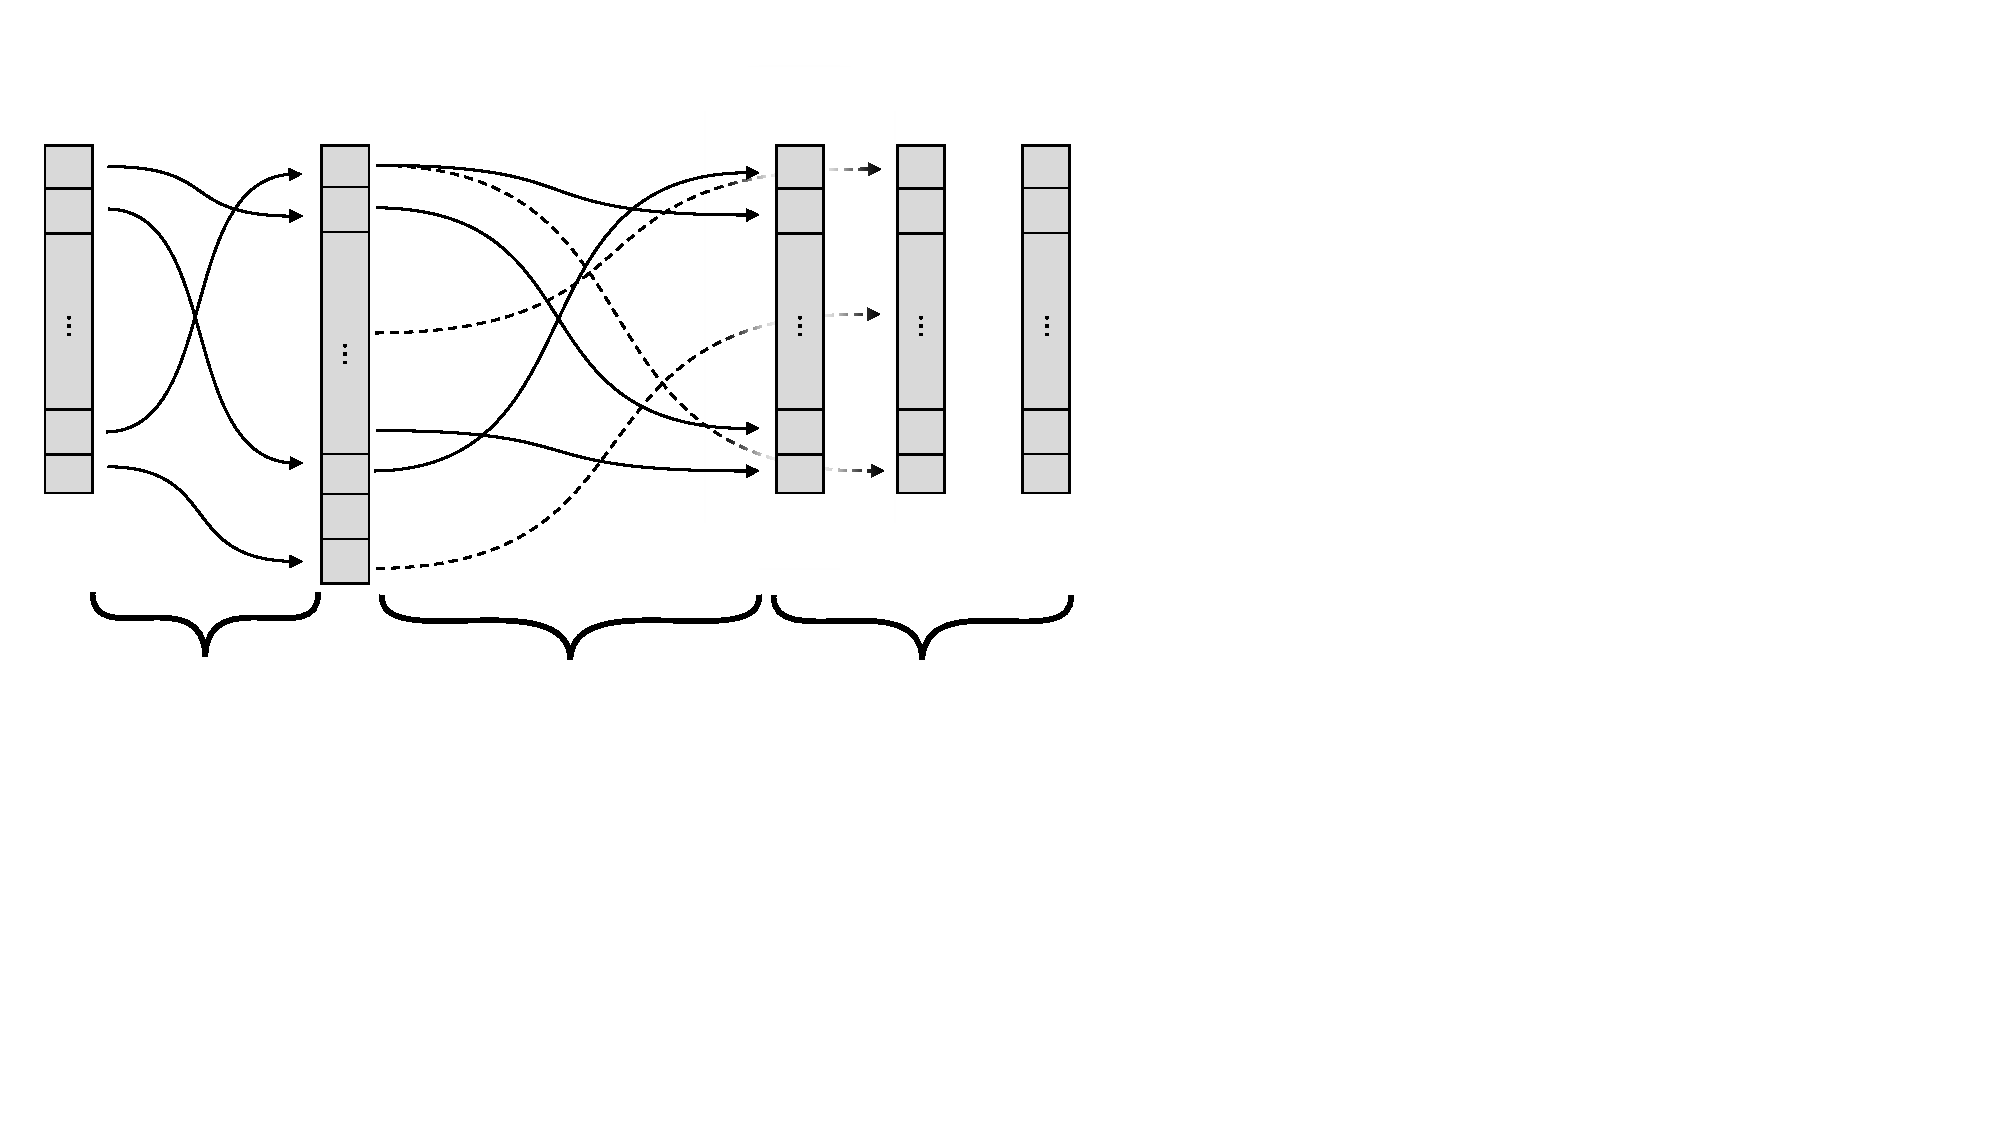
\includegraphics[trim={0cm 7cm 14cm 1cm},clip,width=\textwidth]{diga.pdf}}};
		\draw (-7.9cm,4cm) node {\large$\share{Y}$};
		\draw (7.2cm,4cm) node {\large$X$};
		\draw (-3.7cm,4cm) node {\large$\ytable=\textsf{Cuckoo}(Y)$};
\draw (3.3cm,4cm) node { \large$\widehat{Y}^0$};
		\draw (5.2cm,4cm) node { \large$\widehat{Y}^1$};
		
		\draw (-5.8cm,-4.5cm) node { 1) Cuckoo hash  $Y$  };
		\draw (-5.8cm,-5.0cm) node { using oblv. permutation.};
		\draw (-5.8cm,-5.5cm) node { $\exists j$ s.t. $T[h_j(Y[i])]=Y[i]$. };
		
		
		\draw (-0.3cm,-4.5cm) node { 2) Select Cuckoo locations $T[h_j(X[i])]$  };
		\draw (-0.3cm,-5.0cm) node { using oblv. switching network.};
		\draw (-0.3cm,-5.5cm) node { $\widehat{Y}^j[i]=T[h_j(X[i])]$.};
		
		
		
		\draw (5.4cm,-4.5cm) node { 3) Compare $\widehat{Y}^0[i],\widehat{Y}^1[i]$ w/ $X[i]$};
		\draw (5.4cm,-5.0cm) node { using MPC circuit and  };
		\draw (5.4cm,-5.5cm) node {construct output row. };
		\end{tikzpicture}}
	\vspace{-0.3cm}
	\caption{Overview of the join protocol using oblivious switching network.\label{fig:mapping}}
	\vspace{-0.4cm}
\end{figure}

The main challenge in bringing the described algorithm to the secret shared setting is constructing the cuckoo hash table $\ytable$ and selecting rows from $\ytable$ without leaking sensitive information. We achieve this with the use an MPC friendly \emph{randomized encoding} and a new three-party protocol called an \emph{oblivious switching network}.


Let us continue to assume that the columns $X_1$ and $Y_1$ are the join-keys. Our protocol begins by generating a \emph{randomized encoding} for each of the secret shared join-key $\share{x_i}\in \share{X_1}$ and $ \share{y_i}\in \share{Y_1}$. \figureref{fig:randomized-encode-ideal} contains the ideal functionality for this encoding which takes secret shares from the parties, apply a PRF $F_k$ to the reconstructed value using a internally sampled key $k$, and returns the resulting value to one of the three parties. For $\share{ x_i}:= \share{X_1}[i]$, \Party{0} will learn $F_k(x_i)$ while \Party{1} will learn $F_k(y_i)$ for $\share{ y_i}:=\share{Y_1}[i]$. Since the join-keys $x_i$ (resp. $y_i$) are unique and $k$ is not known, this can be simulated by sending random values to \Party{0} (resp. \Party{1}).

Party \Party{1} proceeds by constructing a \emph{secret shared} cuckoo hash table $\shareTwo{\ytable}$ from the rows of $\share{Y}$ where the hash function values for row $i$ are defined as $h_j(y_i) = H( j || F_k(y_i))$. Note that \Party{1} knows only the randomized encodings $F_k(y_i)$ of each row $Y[i]$, and not the contents of the row itself. The goal in this step is to construct a secret shared cuckoo table $\shareTwo{\ytable}$ such that row $Y[i]$ is located at $\ytable[h_j(y_i)]$ for some $j$. We construct  $\shareTwo{\ytable}$ using a three-party \emph{oblivious permutation protocol} where \Party{1} inputs a permutation $\pi$, all parties input secret shares of $Y$, and the result is secret shares of ``$Y$ permuted according to $\pi$'' which forms $\ytable$ (details follow later). This completes \stepref{step:overview1} and is the first transformation shown in \figureref{fig:mapping}.

It is now the case that $\shareTwo{\ytable}$ is a valid cuckoo hash table of $\share Y$ which is secret shared between \Party{0} and \Party{1}. Party \Party{0}, who knows the randomized encodings $F_k(x_i)$ for all $\share{ x_i}:= \share{X_1}[i]$, now must compare the rows of $\shareTwo{\ytable}$ indexed by $h_j(x_i)= H( j || F_k(x_i))$ with the row $\share X[i]$. In particular, assuming we use two cuckoo hash functions, then \Party{0} constructs two \emph{oblivious switching networks} that maps the shares $\shareTwo{\ytable[{h_0(x_i)}]}$ and $\shareTwo{\ytable[{h_1(x_i)}]}$ to be ``aligned" with $\share X[i]$. Exactly how such a network operates is discussed later but the result is two new tables $\shareTwo{\widehat{Y}^0},\shareTwo{\widehat{Y}^1}$ such that $\ytable[{h_j(x_i)}]=\widehat{Y}^j[i]$. This completes \stepref{step:overview2} and is the second transformation shown in \figureref{fig:mapping}.

Once the shares of $\widehat{Y}^0[i]={\ytable[{h_0(x_i)}]}, \widehat{Y}^1[i]={\ytable[{h_1(x_i)}]}$ are obtained using the switching network, the parties employ an MPC protocol to directly compare these rows with $\share{X}[i]$. That is, they compute a bit $\share{b}$ which equals one if the join-keys are equal and the \texttt{where} clause $P(\shareTwo{\widehat{Y}^j}[i],\share{X}[i])$ outputs one for some $j$. For each row, the output row for an inner join is constructed as $S(\shareTwo{\widehat{Y}^j}[i],\share{X}[i])$ using MPC where $S$ is the user defined selection circuit. In addition, the MPC circuit outputs the secret shared flag $\share{b}$ indicating whether this row is set to \texttt{NULL}. 

Left joins work in a similar way except that all rows of $X$ are output and marked not \texttt{NULL}. Finally, unions can be computed by including all of $Y$ in the output and all of the rows of $X$ where the comparison bit $\share{b}$ is zero. Regardless of the type of join, the protocols do not reveal any information about the tables. In particular, not even the cardinality of the join is revealed due to the use of \texttt{NULL} rows.

\subsection{Randomized Encodings}\label{sec:encode}

The randomized encoding functionality \f{encode} of \figureref{fig:randomized-encode-ideal} enables the parties to coordinate their secret shares without revealing the underlying values. In particular, the parties will construct a cuckoo hash table using these encodings. The functionality takes as input several tuples $(\share{B_i},\share{X_i},\Party{i})$ where $B_i\in\{0,1\}^d$ is an array of $d$ bits, $ X_i\in(\{0,1\}^\sigma)^{d}$ is a array of $d$ strings and  $\Party{i}$ that denotes that party $\Party{i}$ should be output the encodings for this tuple. The functionality assigns a random $\ell$ bit encoding for each input $x\in \{0,1\}^\sigma$. For $j\in[d]$, if the bit $B_i[j]=0$ then the functionality outputs the encoding for $X_i[j]$ and otherwise a random $\ell$ bit string. Looking forward, $B_i[j]=1$ will mean that the key $X_i[j]$ is actually set to \Null and a random encoding should be returned.



\begin{figure}[ht]
	\framebox{\begin{minipage}{0.95\linewidth}\small
			Parameters: Input string size of $\sigma$ bits and output encoding size of $\ell$ bits.
			
			{\bf [Encode]} Upon receiving command $(\textsc{Encode},$ $\{(\share{B_i},\share{X_i}, \Party{i})\})$ from all parties where $X_i\in (\{0,1\}^\sigma)^{d_i}, B_i\in\{0,1\}^{d_i}$ for some $d_i\in \mathbb{Z}^*$. 
			\begin{enumerate}				
				\item Sample a uniformly random $F:\{0,1\}^\sigma \rightarrow \{0,1\}^\ell$. Define $F':\{0,1\}\times \{0,1\}^\sigma \rightarrow \{0,1\}^\ell$ as  $F'(b,x) = \overline{b}F(x) + br$ where $r\gets\{0,1\}^\ell$ is sampled each call.
				
				\item For each $(\share{ B_i},\share{ X_i},\Party{i})$, send $\{F'(b,x)\mid (b,x)\in \textsc{zip}(B_i,X_i)\}$ to $\Party{i}$. 
			\end{enumerate}
	\end{minipage}}
\vspace{-0.3cm}
	\caption{The Randomized Encoding ideal functionality \f{encode}}
	\label{fig:randomized-encode-ideal}	
	\vspace{-0.3cm}
\end{figure}


\paragraph{LowMC Encodings}
We realize this functionality using the LowMC block cipher\cite{lowmc}. When implemented with the honest majority MPC protocols\cite{highthroughput}, this approach results in extremely high throughput, computing up to one million encodings per second. Once the parties have their secret shared inputs, they sample a secret shared LowMC key uniformly and encrypt each input under that key using the MPC protocol. These encryptions are revealed as the encodings to the appropriate party.


The LowMC cipher is parameterized by a block size $\ell$, keys size $\kappa$, s-boxes per layer $m$ and the desired data complexity $d$. To set these parameters, observe that the adversary only sees a bounded number of block cipher outputs (encodings) per key. As such, the data complexity can be bounded by this value. For our implementation we upper bound the number of outputs by $d= 2^{30}$. The remaining parameters are set to be $\ell\in\{80, 100\}$ and $m=14$ which results in $r=13$ rounds and computational security of $\kappa=128$ bits\cite{lowmc}. The circuit for $\ell=80$ contains 546 \textsc{and} gates (meaning each party will send only 546 bits per encoding).

One issue with the LowMC approach alone is that the input size is fixed to be at most $\ell\in\{80,100\}$ bits. However, we will see that the larger join protocol requires an arbitrary input size $\sigma$. This is accommodated by applying a universal hash function to the input shares. Specifically, the parties jointly pick a random matrix $E\gets\{0,1\}^{\sigma\times \ell}$. The parties can then locally multiply each secret shared input before it is sent into the LowMC block cipher.

The security of this transformation follows from $xE\neq x'E$ with overwhelming probability if $x\neq x'$. In particular, $f(x)=xE$ is a universal hash function given that $E$ is independent of $x$. As such the probability that $f(x)=f(x')$ for any $x\neq x'$  is $2^{-\ell}$. Applying the birthday bound we obtain that probability of any collisions among the tuples is $2^{-\ell+p}$ where $p=\log_2 D^2/2=2\log_2(D)-1$ and $D=\sum_i d_i$ is the total number of encodings.

Conditioned on the inputs to the block cipher being unique, the outputs of the block cipher is also distinct and indistinguishable from random $\ell$ bit strings. As such, in the simulation the real outputs can be replaced with that of the ideal functionality so long as $2^{-\ell+p}$ is statistically negligible, i.e. $\ell-p\geq\lambda$.




\begin{figure}
	\framebox{\begin{minipage}{0.95\linewidth}\small
			Parameters: Input, output size of $\sigma$, $\ell$ bits (respectively). Computational security parameter $\kappa$.
			
			{\bf [Encode]} Upon receiving command $(\textsc{Encode},$ $\{(\share{B_i}, \share{X_i}, \Party{i})\})$ from all parties where each $X_i\in (\{0,1\}^\sigma)^{d_i}$. Let $d=\max_i(d_i)$.
			\begin{enumerate}
				\item If $\sigma >\ell,$ the parties jointly sample a matrix $E\in\{0,1\}^{\sigma\times \ell}$. Otherwise $E$ is the ${\sigma\times \ell}$ identity matrix.
					
				 \item The parties have \f{mpc} evaluate the following circuit:
				\begin{enumerate}				
					\item Uniformly sample a key $k$ for a LowMC cipher with block size $\ell$,  security $\kappa$ and data complexity at least $d$ blocks.
					\item For each $(\share{B_i}, \share{X_i}, \Party{i})$ input pair, reveal $\{ F'(b,x) \mid (b,x)\in \textsc{zip}(B_i, X_i)\}$ to \Party{i} where $F'(b,x)=\textsf{LowMC}_k(xE)\oplus br$ and $r\gets\{0,1\}^\ell$ is sampled for each call.
				\end{enumerate}			
		\end{enumerate}
	\end{minipage}}
\vspace{-0.2cm}
	\caption{The randomized encoding LowMC protocol.}
	\label{fig:randomized-encode-lowMC}	
	\vspace{-0.4cm}
\end{figure}



\subsection{Oblivious Switching Network}

The ideal functionality of a switching network was introduced by Mohassel and Sadeghian\cite{MS13}. It obliviously transform a vector $A=(A_1,...,A_n)$ such that the output is $A'=(A_{\pi(1)}, ..., A_{\pi(m)})$ for an arbitrary function $\pi : [m]\rightarrow[n]$. The accompanying protocol of \cite{MS13} was designed in the two party setting where the first party inputs $A$ while the second party inputs a description of $\pi$. \iffullversion
This switching network require  $O(n\log n)$ cryptographic operations. Building on this general paradigm, we 
\else 
We
\fi
introduce a \emph{new} oblivious switching network protocol tailored for the honest majority setting with significantly efficiency improves. Our protocol has $O(n)$ overhead and is constant round. \cite{MS13} requires $O(n\log n \kappa)$ communication/computation and $O(\log n)$ rounds. 
\newcommand{\programmer}{\ensuremath{P_{\textsf{p}}}\xspace}
\newcommand{\sender}{\ensuremath{P_{\textsf{s}}}\xspace}
\newcommand{\receiver}{\ensuremath{P_{\textsf{r}}}\xspace}

The ideal functionality of our protocol is given in \figureref{fig:perm-ideal} with three parties, a programmer \programmer, a sender \sender and a receiver \receiver. \programmer has a description of  $\pi$ while \programmer,\sender have a secret sharing of a vector $A\in \Sigma^n$ where $\Sigma=\{0,1\}^\sigma$.  \programmer and  \receiver are each output a share of $\shareTwo{A'}$ s.t. $A'=(A_{\pi(1)}, ..., A_{\pi(m)})$. For ease of presentation, we will initially assume $A$ is the private input of \sender. 

\begin{figure}\small
	\framebox{\begin{minipage}{0.95\linewidth}


			Parameters: $3$ parties denoted as the \programmer, \sender and \receiver. Elements are strings in $\Sigma:=\{0,1\}^\sigma$. An input vector size of $n$ and output size of $m$.
			
			{\bf [Switch]} Upon the command $(\textsc{switch}, \pi, \shareTwo{A}_0)$ from the \programmer and $(\textsc{switch}, \shareTwo{A}_1)$ from the \sender:
			\begin{enumerate}
				\item Interpret $\pi: [m]\rightarrow [n]$ and $A\in \Sigma^n$. 
				\item Compute $A'\in \Sigma^m$ s.t. $\forall i\in [m], A_{\pi(i)} = A'_i$.
				\item Generate $\shareTwo{A'}$ and send $\shareTwo{A'}_0$ to \programmer and $\shareTwo{A'}_1$ to \receiver.
			\end{enumerate}
 	\end{minipage}}
	\vspace{-0.2cm}
	\caption{The Oblivious Switching Network ideal functionality \f{Switch}. See \figureref{fig:perm-ideal-2}, \ref{fig:dup-ideal-2} for \f{Permute} and \f{Duplicate}.}
	\label{fig:perm-ideal}	
	\vspace{-0.5cm}
\end{figure}


\paragraph{Permutation Network}\label{sec:perm}
We begin with a restricted class of switching networks where the programming function $\pi$ is injective. {That is, each input element $A_i$ will be mapped to a maximum\footnote{Strictly speaking, this protocol implementation a generalization of a permutation network since it allows some elements to not appear in the output, i.e. $m<n$ and $\pi:[m]\rightarrow[n]$.} of one location in the output $A'$.} As we will see later, this property will simplify the implementation since we do not need to duplicate any element. 
Intuitively, the Permute protocol of \figureref{fig:switching-net} instructs \sender to first   shuffled $A$ in a random order (as specified by $\pi_0$) and then secret share it between \programmer \& \receiver. Then \programmer \& \receiver will reorder these shares (as specified by $\pi_1$) to be in the desired order (i.e. $\pi$). This is done as follows, \programmer samples two random functions $\pi_0,\pi_1$ such that $\pi_1 \circ \pi_0 = \pi$, $\pi_0:[n]\rightarrow [n]$ is bijective and $\pi_1:[m]\rightarrow [n]$ is injective.  \programmer sends   $\pi_1$ to  \receiver and $\pi_0, S\gets \Sigma^{n}$ to  \sender who sends $B := (A_{\pi_0(1)} \oplus S_0, ...,A_{\pi_0(n)} \oplus S_n )$ to  \receiver. The final shares of $A'=\pi(A)$ are defined as  \programmer holding $\shareTwo{A'}_0:=(S_{\pi_1(1)}, ..., S_{\pi_1(m)})$ and the \receiver holding $\shareTwo{A'}_1:=(B_{\pi_1(1)}, ..., B_{\pi_1(m)})$. 

The simulation of this protocol is perfect. The view of \sender contains a uniform permutation $\pi_0$ and vector $S$.  Similarly, the view of  \receiver contains $\pi_1$ which is uniformly distributed (when $\pi_0$ is unobserved) and the uniform vector $B$. See \sectionref{sec:perm-proof} for details.
In our computational secure setting,  $\pi_0,S$ can be generated locally by \programmer and \sender using a common source of randomness, e.g. a seeded PRG. This reduces the rounds to 1.  


\paragraph{Shared Inputs} As presented here in the text our protocols assume the input vector $A$ being transformed is the private input of the \sender. However, the full protocols will require the input $A$ to secret shared. Let us assume we have some switching network protocol $\Pi$ which takes input $A$ from \sender, $\pi$ from \programmer and output shares of $\pi(A)$. Then this can be transform to shared input $\shareTwo{A}$. The parties invoke $\Pi$ where \sender input their share $\shareTwo{A}_1$ and \programmer inputs $\pi$. \programmer and \receiver receive $\shareTwo{B}$ from the functionality. The final result can then be computed as \receiver holding $\shareTwo{A'}_1:=\shareTwo{B}_1$ while \programmer  locally defines $\shareTwo{A'}_0:=\shareTwo{B}_0\oplus \pi(\shareTwo{A}_0)$. It is easy to verify that $A'=\pi(\shareTwo{A}_1)\oplus \pi(\shareTwo{A}_0)=\pi(A)$. The protocol descriptions in \figureref{fig:switching-net} include this shared input modification. However, here in the text we will continue to assume $A$ is the sole input of \sender.


\begin{figure}
	\framebox{\begin{minipage}{0.95\linewidth}\small
			Parameters: $3$ parties denoted as \programmer, \sender and \receiver. Elements are strings in $\Sigma:=\{0,1\}^\sigma$. An input, output vector size of $n, m$.
			\smallskip
			
			{\bf [Permute]} Upon the command $(\textsc{Permute}, \pi, \shareTwo{A}_0)$ from  \programmer and $(\textsc{Permute}, \shareTwo{A}_1)$ from  \sender. Require that $\pi: [m]\rightarrow [n]$ is \emph{injective} and  $\shareTwo{A}_0,\shareTwo{A}_1\in \Sigma^{n}$. Then:
	\begin{enumerate}[leftmargin=.5cm]
		\item  \programmer uniformly samples a bijection $\pi_0 : [n]\rightarrow[n]$ and  let $\pi_1 :[n] \rightarrow[m]$ s.t. $\pi_1\circ \pi_0 = \pi$.  \programmer sends $\pi_0 $ and  $S\gets \Sigma^{n}$  to  \sender.
		\item  \sender sends $B := ( \shareTwo{A_{\pi_0(1)}}_1 \oplus S_1, ...,  \shareTwo{A_{\pi_0(n)}}_1 \oplus S_n)$ to  \receiver.
		\item  \programmer sends $\pi_1$ and $T\gets\Sigma^{m}$ to  \receiver who outputs $\shareTwo{A'}_0:=\{B_{\pi_1(1)} \oplus T_1,...,B_{\pi_1(m)}\oplus T_m\}$.  \programmer outputs $\shareTwo{A'}_1:=\{ S_{\pi_1(1)}\oplus T_1\oplus  \shareTwo{A_{\pi(1)}}_0,...,S_{\pi_1(m)}\oplus T_m\oplus \shareTwo{A_{\pi(m)}}_0\}$.
	\end{enumerate} 			

{\bf [Duplicate]} Upon the command $(\textsc{Duplicate}, \pi, \shareTwo{A}_0)$ from  \programmer and $(\textsc{Duplicate}, \shareTwo{A}_1)$ from  \sender. Require that $\pi: [n]\rightarrow [n]$ s.t $\pi(1)=1$ and $ \pi(i)\in \{i,\pi(i-1)\}$ for $i\in [2,n]$ and  $A\in\Sigma^{n}$. Then:
\begin{enumerate}[leftmargin=.5cm]
	
	\item  \programmer  computes the vector $b\in\{0,1\}^{m}$ such that $b_1=0$ and for $i\in[2,n],$ $b_i=1$ if $\pi(i)=\pi(i-1)$ and 0 otherwise.
	
	\item \sender samples $\shareTwo{B}_1, W^0,W^1\gets \Sigma^{n}, \shareTwo{B_1}_0\gets\Sigma$ and $\phi\gets\{0,1\}^n$. \sender redefine $\shareTwo{B_1}_1:=\shareTwo{A_1}_1\oplus \shareTwo{B_1}_0$. For $i\in [2,n]$, \sender sends 
	\begin{align*}
	M^0_i&:= \shareTwo{A_i}_1 \ \ \ \oplus \shareTwo{B_i}_1 \oplus W^{\phi_i}_i\\
	M^1_i&:= \shareTwo{B_{i-1}}_1 \oplus \shareTwo{B_i}_1 \oplus W^{\overline{\phi_i}}_i
	\end{align*}
	and $\shareTwo{B_1}_0,\phi$ to  \programmer. \sender sends $\shareTwo{B}_1,W^0, W^1$ to  \receiver.  
	\item\programmer sends $\rho:=\phi\oplus b, R\gets\Sigma^n$ to  \receiver who responds with $\{ W^{\rho_i}_i : i\in [2,n] \}$. For $i\in [2,n]$, \programmer defines
	$$
		\shareTwo{B_i}_0:= M^{b_i}_i \oplus W^{\rho_i}_i\oplus b_i\shareTwo{B_{i-1}}_0
	$$
	\programmer outputs $\shareTwo{A'}_0:=\shareTwo{B}_0\oplus R\oplus \pi(\shareTwo{A}_0)$ and \receiver outputs $\shareTwo{A'}_1:=\shareTwo{B}_1\oplus R$.
\end{enumerate} 			
				{\bf [Switch]} Upon the command $(\textsc{Switch}, \pi, \shareTwo{A}_0)$ from  \programmer and $(\textsc{Switch}, \shareTwo{A}_1)$ from  \sender where $\pi: [m]\rightarrow [n]$ and $\shareTwo{A}_0,\shareTwo{A}_1\in \Sigma^{n}$. 
				\begin{enumerate}[leftmargin=.5cm]
					
					\item  \programmer samples an injection $\pi_1:[m]\rightarrow [n]$ s.t. for $i\in image(\pi)$ and $k=|preimage(\pi, i)|$,  $\exists j$ where $\pi_1(j)=i$ and $\{\pi_1(j+1), ...,\pi_1(j+k) \}\cap image(\pi)=\emptyset$. 
					 \programmer  sends $(\textsc{Permute}, \pi_1, \shareTwo{A}_0)$ to \f{Permute} and  \sender sends $(\textsc{Permute}, \shareTwo{A}_1)$.  \programmer receives $\shareTwo{B}_{0}\in \Sigma^{m}$ in response and  \receiver receives $\shareTwo{B}_{1}\in \Sigma^{m}$. 
					
					\item  \programmer defines $\pi_2:[m]\rightarrow[m]$ s.t. for $i\in image(\pi)$ and $k:=|preimage(\pi, i)|$ and $j$ where $\pi_1(j)=i$, then $\pi_2(j)=...=\pi_2(j+k)=j$. \programmer and \receiver respectively send $(\textsc{Duplicate}, \pi_2, \shareTwo{B}_0)$ and $(\textsc{Duplicate}, \shareTwo{B}_{1})$ to \f{Duplicate}. As a result \programmer obtains $\shareTwo{C}_0\in \Sigma^m$ from \f{Duplicate} and \sender obtains $\shareTwo{C}_1\in \Sigma^m$.
					
					\item \programmer computes the permutation $\pi_3:[m]\rightarrow[m]$ such that for  $i\in image(\pi)$ and $k=|preimage(\pi, i)|$, $\{\pi_3(\ell) : \ell\in preimage(\pi, i)\}=\{j, ..., j +k\}$ where $i=\pi_1(j)$.	 \programmer sends $(\textsc{Permute}, \pi_3, \shareTwo{C}_0)$ to \f{Permute} and  \sender sends $(\textsc{Permute},\shareTwo{C}_1)$.  \programmer receives $S\in \Sigma^{m}$ in response. \programmer and \receiver respectively receives and outputs $\shareTwo{A'}_0,\shareTwo{A'}_1\in \Sigma^{m }$.
				\end{enumerate} 			
%
 	\end{minipage}}
	\vspace{-0.2cm}
	\caption{The Oblivious Switching Network protocols \proto{Permute}, \proto{Duplicate}, \proto{Switch}. }
	\label{fig:switching-net}	
	\vspace{-0.4cm}
\end{figure}


\paragraph{Duplication Network}\label{sec:dup}

The Duplication protocol of \figureref{fig:switching-net} considers a second type of restricted network where $\pi : [n]\rightarrow[n]$, s.t.  $\pi(1)=1$ and $\pi(i)\in \{i, \pi(i-1)\}$ for $i=2,...,n$. That is, each output position is either a copy of the same input position (i.e. $\pi(i)=i$) or is a duplicate of the previous output position (i.e. $\pi(i)=\pi(i-1)$). For example, let the truth table of $\pi$ be $(\pi(1),...,\pi(6))=(1,1,3,4,4,4)$ and therefore $A'=(A_1,A_1,A_3,A_4,A_4,A_4)$. Note the only change is that $A_1,A_4$ were duplicated into the next position(s). This transformation can be characterized by a vector $b\in\{0,1\}^{n}$ where $b_i=1$ denotes that the output position $i$ should be a copy of output position $i-1$, i.e. $b=(0,1,0,0,1,1)$ for the example above. Therefore we get the relation $A'_i=\overline{b_i}A_i \oplus b_iA_{i-1}'$ for $i\in[2,n]$. 

As a warm-up, let us fix some index $i$ and consider the simpler relation where 
$$
	A'_i=\overline{b_i}A_i \oplus b_iA_{i-1},
$$
i.e. $A_i'$ is either $A_i$ or $A_{i-1}$ and not $A_{i-1}'$ as described before. Conceptually, we will implement this using an OT-like protocol with  OT messages $(A_i,A_{i-1})$ and select-bit $b_i$. \sender samples three uniform strings $\shareTwo{A'_{i}}_1, w_0,w_1\gets \Sigma$ and a uniform bit $\phi\gets \{0,1\}$. \sender constructs two messages $m_0=A_{i}\oplus \shareTwo{A'_{i}}_1\oplus w_\phi$ and $m_1= A_{i-1}\oplus \shareTwo{A'_{i}}_1 \oplus w_{\phi\oplus 1}$.  \sender sends $w_0,w_1$ to  \receiver and sends $m_0,m_1,\phi$ to  \programmer who sends $\rho=\phi\oplus b_i$ to  \receiver. The final shares\footnote{Due to technique reasons about simulating output the full protocol  additionally randomizes the output shares. } are constructed by having  \receiver send $w_\rho$ to  \programmer
 who computes $\shareTwo{A'_{i}}_0:=m_{b_i}\oplus w_{\rho}$. In our computationally secure setting observe that sending $w_0,w_1,\phi$ can be optimized away using a seed.
 



The protocol just described considers the setting where the parties select between $A_{i},A_{i-1}$. However, we require that at each iteration the messages being selected is either $A_{i}$ or $A'_{i-1}$ where $\shareTwo{A_{i-1}'}$ was computed in the previous iteration. Fortunately this can be achieved at no overhead by leveraging that fact that \programmer knows $b_i$ and $\shareTwo{A'_{i-1}}_0$ ahead of time. At index $i$, \sender uses $\shareTwo{A'_{i-1}}_1$ instead of $A_{i-1}$ while the \programmer computes $\shareTwo{A'_{i}}_0:=m_{b_i}\oplus w_{\rho}\oplus b_i\shareTwo{A'_{i-1}}_0$. As such, \programmer is manually adding other other share of $\shareTwo{A'_{i-1}}$ when it is need. The full proof of security is in \sectionref{sec:dup-proof}.  To briefly show correctness, let us assume by induction that $\shareTwo{A'_{i-1}}$ is correct, then:
{\small
\begin{align*}
A'_i&=(m_{b_i}\qquad\qquad\qquad\qquad\qquad\qquad\quad\ \, \, \oplus w_{\rho}\oplus b_i\shareTwo{A'_{i-1}}_0) \oplus (\shareTwo{A'_i}_1)\\
	&=(\overline{b_i}A_i\oplus b_i\shareTwo{A'_{i-1}}_1 \oplus \shareTwo{A'_{i}}_1\oplus w_{b_i\oplus\phi}\oplus w_{\rho}\oplus b_i\shareTwo{A'_{i-1}}_0) \oplus (\shareTwo{A'_i}_1) \\
	&=\overline{b_i}A_i \oplus b_i A'_{i-1}
\end{align*}}
\vspace{-0.4cm}


\paragraph{Universal Switching Network}\label{sec:switch}
Our Switch protocol of \figureref{fig:switching-net} is a universal switching network for an \emph{arbitrary}  $\pi : [m]\rightarrow [n]$ and is constructed in three phases\cite{MS13}:
 $A\overset{\pi_1}{\rightarrow}B\overset{\pi_2}{\rightarrow}C\overset{\pi_3}{\rightarrow}A'=\pi(A)$. 
 
 Let us first work through an example $\pi[6]\rightarrow[8]$ where $(\pi(1),...,$ $\pi(6))=(4,3,4,7,4,7)$. Observe that $4$ appears three times, $7$ appears twice and $\{1,2,5,6,8\}$ are ``unused''. First we apply the permutation $B=\pi_1(A)$ which ensures $A_4$ is followed by two unused elements and $A_7$ is followed by one, e.g. $B=(A_3,A_4,A_1,A_2,A_7,A_8)$. In general, an element that should appear $k>1$ times will be followed by $k-1$ unused elements. Note that $|B|=|A'|$ and need not be the size of $A$. This is achieved by dropping some unused elements, e.g. $A_5,A_6$. The duplication network $C=\pi_2(B)$ will duplicate $A_4$ twice and $A_7$ once, e.g. $C=(A_3,A_4,A_4,A_4,A_7,A_7)$. Note that only elements in $A'$ are left now and they have the correct multiplicity. Finally, $A'=\pi_3(C)$ permutes $C$ to be in the desired order, e.g. $A'=(A_4,A_3,A_4,A_7,A_4,A_7)$.
 
More specifically, the transformations are defined as:
\begin{enumerate}
	\item $B:=\pi_1(A)$: Sample an injective $\pi_1:[m]\rightarrow[n]$ s.t. if $\pi$ maps an input position $i$ to $k$ outputs positions (i.e. $k=|preimage(\pi,i)|=|\{ j : \pi(j)=i \}|$), then there exists a $j$ such that $\pi_1(j)=i$  and $\{\pi_1(j+ 1),...,\pi_1(j +k-1)\} \cap image(\pi) = \emptyset$. 
	
	\item $C:=\pi_2(B)$: Let $\pi_2:[m]\rightarrow[m]$ s.t. if $A_i$ is mapped to $k>0$ positions in $A'=\pi(A)$, then for $\pi_1(j)=i$ it holds that $ C_{j}=...=C_{j+k-1} = A_i=B_j$. That is, $\pi_2(j)=...=\pi_2(j+k-1)=j$.
	
	\item $A':=\pi_3(C)$: Sample permutation $\pi_3:[m]\rightarrow[m]$  s.t. $C$ is permuted to the same ordering as $\pi(A)$. That is, for $i\in image(\pi)$ and $\pi_1(j)=i$, sample permutation $\pi_3$ s.t. $\{\pi_3(\ell)\mid \ell\in preimage(\pi,i)\} =\{j,...,j+| preimage(\pi,i)|-1\}$.
	
\end{enumerate}

Observe that steps $\pi_1,\pi_3$ can both be implemented using the oblivious permutation protocol while $\pi_2$ can be implemented with a duplication network. \figureref{fig:switching-net} provides a formal description of the full switching network protocol. The simulation of this protocol is presented in \sectionref{sec:switch-proof} and follows from the simulation of the permutation and duplication subprotocols. 

\paragraph{Comparison}
We compare with alternative constructions to illustrate the performance improvement that our switching protocol provides. The first and most traditional is for $\sender$ to use additive homomorphic encryption, e.g. Paillier, to encrypt the shares $\shareTwo{A}_1$ and send these to \programmer. \programmer can apply the mapping function $\pi$ to these encryptions, rerandomize them and send the result back to \sender who decrypts it to obtain their share of $\shareTwo{A'}_1$. This approach has a very high computational overhead compared to ours due to additive homomorphic encryption being an intensive process. 

An alternative approach is that taken by \cite{MS13} which can be viewed as the two party version of our protocol. In their setting the permutation network is the most expensive operation and is implemented using $O(n\log n)$ OTs\cite{C:IKNP03}. Our protocol is both asymptotically more efficient by a $O(\log n)$ factor and has smaller constants since our protocol does not require the relatively more expensive OT primitive. 

\subsection{Join Protocols}\label{sec:join}

Our join protocol can be divided into four phases:

\begin{enumerate}
	\item Compute randomized encodings of the join-columns/keys. 
	\item Party \Party{1} constructs a cuckoo table $T$ for table $Y$ and arranges the secret shares using a permutation protocol. 
	\item For each row $x$ in $X$, \Party{0} uses an oblivious switching network to map  the corresponding location $i_1,i_2$ of the cuckoo hash table to a secret shared tuple $(x, T[{i_1}], T[{i_2}])$.
	\item The join-key(s) of $x$ is compared to that of $T[{i_1}], T[{i_2}]$. If one of them match then the corresponding $Y'$ row is populated; otherwise the $Y'$ row is set to \texttt{NULL}.
	\item The various types of joins can then be constructed by comparing row $i$ of $X$ and $Y'$.
\end{enumerate} 
Steps 1 through 4 are performed by the Map routine of \figureref{fig:full_proto} while step 5 is performed in the Join routine. \figureref{fig:full_ideal} contains the ideal functionality of the join protocol.



\paragraph{Randomized Encodings.}
We begin by generating randomized encodings of the columns being used for the join-keys. For example, 
\iffullversion
$$
	\texttt{select }* \texttt{ from } X \texttt{ inner join } Y \texttt{ on } X_1 = Y_1 \texttt{ and } X_2 = Y_3
$$

\else
selecting all columns of $X$ and $Y$ where $X_1 = Y_1 \texttt{ and } X_2 = Y_3$.
\fi
In this case there are two join-keys, $X_1,X_2$ from $X$ and $Y_1,Y_3$ from $Y$. The protocol has \Party{0} learn the randomized encoding for each row of $X$ and \Party{1} learn them for $Y$. Importantly, is that after a previous join operation, some (or all) of the rows being joined can be \texttt{NULL}. We require that the randomized encodings of these rows not reveal that they are \texttt{NULL}. For table $X$, a special column $\XNull$ encodes if for each row is logically \texttt{NULL}. The \f{encode} functionality will then return a random encoding for all \texttt{NULL} rows. Specifically, the parties will send $(\textsc{Encode}, \{(\share{\XNull}, \share{X_{j_1}||...||X_{j_l}}, \Party{0}), (\share{\YNull}, \share{Y_{k_1}||...||$ $Y_{k_l}}, \Party{1})\})$ to \f{encode} where $j_1,...,j_l$ and $k_1,...,k_l$ index the join-keys of $X$ and $Y$. Let $\mathbb{E}_x,\mathbb{E}_y\in(\{0,1\}^{\ell})^n$ be the encodings that \Party{0} and \Party{1} respectively receive from \f{encode}.


For correctness, we require the encoding bit-length $\ell$ to be sufficiently large such that the probability of a collision between encodings is statistically negligible. Given that there are a total of $D=2n$ encodings, the probability of this is at most $2^{-\ell+2\log_2 D-1}$ which we require to be less than $2^{-\lambda}$, therefore $\ell\geq \lambda+2\log_2 D -1$. Our implementation uses $\lambda=40$ and $\ell\in\{80,100\}$ depending on $D$.




\paragraph{Constructing the Cuckoo Table.}
The next phase of the protocol is for \Party{1} to construct a secret shared cuckoo table for $Y$ where each row is inserted based on its encoding in $\mathbb{E}_y$. \Party{1} locally inserts the encodings $\mathbb{E}_y$ into a plain cuckoo hash table $t$ with $m\approx1.5n$ slots using the algorithm specified in \sectionref{sec:prelim} and \cite{DRRT18}. In the presentation we assume two hash functions are used. \Party{1} samples an injective function $\pi : [m]\rightarrow [m]$ such that  $t[j]=\mathbb{E}_y[i]$, then $\pi(j)=i$.
\iffullversion
 That is, $\pi$ defines the mapping from each row's original position in the table $Y$ to the corresponding position in the cuckoo table $t$.
\fi

Parties \Party{0} and \Party{1} convert $\share{Y}$ to $\shareTwo{Y}$ such that \Party{0} holds $\shareTwo{Y}_0$. 
\Party{1} sends $(\textsc{Switch}, \pi, \shareTwo{Y}_1)$ to \f{switch} and \Party{0} sends $(\textsc{Switch}, \shareTwo{Y}_0)$.
In response \f{switch} sends $\shareTwo{\ytable}_{1}$ to \Party{1}  and $\shareTwo{\ytable}_{0}$ to \Party{2}. 
It is now the case that $\ytable$ is a valid secret shared cuckoo hash table of $Y$.
\iffullversion
 In particular, for a given row $Y[i]$ with encoding $e=\mathbb{E}_y[i]$, there exists a $j\in \{h_1(e),h_2(e)\}$ such that  $\ytable[j] = Y[i]$. Here, the $h_0,h_1$ functions are hash functions used to construct the cuckoo table $\ytable$. Another important observation is that $\pi$ is a permutation and therefore the more efficient permutation protocol can be used in place of the universal switching protocol.

We note that some of the columns of the tables may be secret shared in arithmetic group as opposed to binary shares. In this case the switching network will use the appropriate arithmetic operation as note in \sectionref{sec:switch}. 
\fi

\paragraph{Selecting from the Cuckoo Table.}
The next phase of the protocol is for each row of $X$, select the appropriate rows of $\ytable$ so the keys can be compared. \Party{0} knows that if the join-keys of the $X[i]$ row will match with a row from $Y$, then this row will be at $\ytable[j]$ for some $j\in \{h_1(e),h_2(e)\}$ where  $e=\mathbb{E}_x[i]$. 

To obliviously compare these rows, \Party{0} will construct two switching networks with programming $\pi_1,\pi_2 : [n]\rightarrow [m]$ such that if $h_l(\mathbb{E}_x[i])=j$ then $\pi_l(i)=j$. Each of these will be used to construct the tables $\shareTwo{\widehat{Y}^1},\shareTwo{\widehat{Y}^2}$ which are the result of applying the switching networks $\pi_1,\pi_2$ to $\shareTwo{\ytable}$. For $i\in[n],$ the parties select either $\shareTwo{\widehat{Y}^1}[i]$ or $\shareTwo{\widehat{Y}^2}[i]$ and assign it to $\share{Y'}[i]$ based on which has matching joins keys with $\share{X}[i]$. If there is no match then $\share{Y'}[i]=\Null.$

\paragraph{Inner Join.}
Given the secret shared tables $\share{X},\share{Y'}$ as described above, the parties do a linear pass over the $n$ rows to construct the join between $X$ and $Y$. Recall that the inner join consists of all the selected columns from the rows $X[i],Y[j]$ where  the join-keys of the rows $X[i]$ and $Y[j]$ are equal. 

If row $X[i]$ has a matching row in $Y$ then this row will have been mapped to $Y'[i]$. Next, the \texttt{where} clause further filters the output table as a function of $Y'[i]$ and $X[i]$. 
\iffullversion
For example, the query may specify that only rows where $Y_2'[i] + X_3[i] > 22$  are to be selected. Regardless of the exact where clause, the 
\else 
The
\fi
MPC protocol sets the \texttt{NULL}-bit of the final output table $Z$ as $\ZNull[i] :=\XNull[i] \vee \YNull'[i] \vee \neg  P(Y'[i], X[i])$ where $P$ is the predicate function specified by the \texttt{where} clause.
Finally, the computation specified by the \texttt{select} query is performed, e.g. copying the columns of $X,Y$ or computing a function of them. 


\iffullversion
\paragraph{Optimizations.}
Several optimizations can be applied to this protocol. First, observe that only columns of $Y$ which explicitly appear in the query need to be input to the switching networks. This reduces the amount of data to be sent and improves performance. Secondly, when comparing the join-columns, instead of computing the equality circuit between all of these columns it suffices to compare the randomized encodings. In the event that the join-column(s) contain many bits, comparing the encodings can reduce the size of the equality circuit. In addition, observe that including columns from $X$ in the output table is essentially free due to these secret share columns simply being copied from $X$. Leveraging this the queries can be optimized by ensuring that the majority of the output columns are taken from $X$. Moreover, if a join-column from $Y$ is in the \texttt{select} clause, this output column can be replaced with the matching column in $X$.

Also observe that the computation perform heavily lends itself to SIMD instructions. That is, the same computation is repeatedly applied to each row of the output table. Modern MPC protocol such as the ABY$^3$ framework \cite{aby3,highthroughput} are optimized for this setting and can process billions of binary circuit gates per second\cite{highthroughput}. In addition the ABY$^3$ framework can switch between using binary and arithmetic circuits based on which is most efficient for the given computation. 
\fi

\paragraph{Left/Right Join.}
A left join query is similar to an inner join except that all of the rows from the left table $X$ are included. All rows that are in the inner join are computed as before. For rows only in $X$, the bit $\YNull'[i]$ will equal one and is used to initialize the missing columns from $Y$ to a default, typically \texttt{NULL}. A right join can be implemented symmetrically.

\paragraph{Union and Set Minus.}
Our framework is also capable of computing the union of two tables with respect to the join-keys. Specifically, we define the union operator as taking all of the rows from the left table and all of the rows from the right table that would not be present in the inner join. First we compute $Y\backslash X$ by only including $X[i]$ if $Y'[i]$ is \Null, i.e. $X[i]$ has no matching row in $Y$. The union of $X$ and $Y$ is then constructed as $(Y\backslash X) || X$ where the $||$ operator denotes the row-wise concatenation of $X$ to the end of $Y\backslash X$.


\paragraph{Full Join.}
We construct a full join as $(X$ left join $Y)$ union $Y$. The left join merge the rows in the intersection and the union includes the missing rows of $Y$. The overhead of this protocol is effectually twice that of the other protocols. 

We note that under some restrictions on the tables being joined, a more efficient protocol for full joins can be achieved. We defer an explanation of this technique to \sectionref{sec:threatlog}.

\paragraph{Security.} The simulation of these protocols directly follow from the composibility of the subroutines \f{encode}, \f{switch} and \f{mpc}. First, the output of \f{encode} simply outputs random strings and it is therefore straightforward to simulate.  \f{switch} and \f{mpc} both output secret shared values. Finally, correctness is straight forward to analysis and holds so long as there is no encoding collisions and cuckoo hashing succeeds. Parameters are chosen appropriately so these failure events happen with probability at most $2^{-\lambda}$. See \ref{sec:join-proof} for a full proof of security.

\begin{figure}
	\framebox{\begin{minipage}{0.95\linewidth}
			Parameters: Table size $n$. For all command, $X,Y$ are tables and $\{X_j \mid j\in J\}$ and $\{Y_k \mid k\in K\}$ are the join-keys of $X$ and $Y$ respectively. $S, P$ are resp. the \texttt{select}  and \texttt{where} function.
			
			{\bf [Map]} Upon receiving  $(\textsc{Map},\share{X},J, \share{Y}, K)$ from all parties. \begin{enumerate}[leftmargin=.5cm]
				\item The parties send $(\textsc{Encode}, \{(\share{\XNull}, \share{X_{J_1}||...||X_{J_l}}, $ $\Party{0}), (\share{\YNull}, \share{Y_{K_1}||...||Y_{K_l}}, \Party{1})\})$ to \f{encode} where $l=|J|=|K|$. \Party{0} receives $\mathbb{E}_x$ and \Party{1} receives $\mathbb{E}_y$ from \f{encode}.

				\item \Party{1} constructs a cuckoo hash table $t$ for the set $\mathbb{E}_y$. Define $\pi_0$ such that $\pi_0(j)=i$ where $\mathbb{E}_y[i]=t[j]$.
				
				\item \Party{0} and \Party{1} convert \share{Y} to \shareTwo{Y}. \Party{1} sends $(\textsc{Permute}, \pi_0, \shareTwo{Y}_1)$ to \f{Permute} and \Party{0} sends $(\textsc{Permute}, \shareTwo{Y}_0)$.
				\Party{1} receives $\shareTwo{\ytable}_{1}$ and \Party{2} receives $\shareTwo{\ytable}_{0}$ from \f{Permute}.
				
				\item Let $h_1,...,h_w$ be the cuckoo hash functions. \Party{1} defines $\pi_1,...,\pi_w$ such that $\pi_l(i)=j$ where $h_l(\mathbb{E}_x[i])=j$.
				
				\item For $l\in[w]$, \Party{1} sends $(\textsc{Switch}, \pi_l, \shareTwo{T}_1)$ to \f{Switch} and \Party{2} sends $(\textsc{Switch}, \shareTwo{T}_0)$. \Party{0} receives $\shareTwo{\widehat{Y}^l}_0$ and \Party{1} receives $\shareTwo{\widehat{Y}^l}_1$ from \f{Switch}.
				
				\item For $i\in n$, if $\exists j\in[w]$ s.t. $\widehat{Y}^j_{\Null}[i]=0 \vee \share{X_{J_1}||...||X_{J_l}}[i] = \share{\widehat{Y}^j_{K_1}||...||\widehat{Y}^j_{K_l}}[i]$ then $\share{\widehat{Y}^*}[i]:=\shareTwo{\widehat{Y}^j}[i]$. Otherwise $\share{\widehat{Y}^*}[i]:=(\Null,0,...)$. Output $\share{\widehat{Y}^*}$.
			\end{enumerate}

			{\bf [Join]}  Upon receiving command $(\textsc{Join}, type, \share{X},$ $J, \share{Y}, K, S, P)$ from all parties.
			\begin{enumerate}[leftmargin=.5cm]
				\item The parties send $(\textsc{Map},\share{X},J, \share{Y}, K)$ to \proto{map} and receive $\share{{Y'}}$.
								
				\item Output the table $\share{Z}$ defined by the case $type$:
				\begin{enumerate}[leftmargin=0.6cm]
					\item[$\textsc{Inner}$:] For $i\in [n],$  \f{mpc} evaluate $\share{\ZNull}[i]:=\share{\XNull}[i] \vee \share{\YNull'}[i] \vee \neg P(\share{X}[i], \share{Y'}[i])$ and $\share{Z}[i]:=S(\share{X}[i], \share{Y'}[i])$.
					
					
					\item[$\textsc{Left}$:]
					For $i\in [n],$ \f{mpc} evaluate $\share{\ZNull}[i]:=\share{\XNull}[i] \vee \neg P(\share{X}[i], \share{Y'}[i])$ and $\share{Z}[i]:=S(\share{X}[i], \share{Y'}[i])$.
					
					
					\item[$\textsc{Union}$:] 
					For $i\in [n],$ \f{mpc} evaluate $\share{\ZNull}[i]:= \share{\XNull}[i] \vee \neg P(\share{X}[i], \Null)$ and $\share{Z}[i]:=S(\share{X}[i], \Null)$. 
					
					For $i\in [n],$ \f{mpc} evaluate $\share{\ZNull}[n+i]:= \share{\YNull}[i] \vee \neg \share{\XNull}[i] \vee \neg P(\Null, \share{Y'}[i])$ and $\share{Z}[n+i]:=S(\Null, \share{Y'}[i])$.
					
					\item[$\textsc{Full}$:] all parties sending $(\textsc{Join},$ $\textsc{Left},$ $\share{X},$ $J, \share{Y}, K,$ $S', P)$ to $\proto{join}$ and receiving $\share{X'}$ in response. They then send $(\textsc{Join}, \textsc{Union}, \share{X'}, J, \share{Y}, K, S'', P')$  to $\proto{join}$ and output the response, where $S',S''$ and $P'$ are appropriately updated version of $S,P$.
				\end{enumerate}
				 

			\end{enumerate}
	\end{minipage}}
\vspace{-0.3cm}
	\caption{Join protocols $\proto{map}$ and $\proto{join}$.}
	\label{fig:full_proto}	
	\vspace{-0.3cm}
\end{figure}



\begin{figure}
	\framebox{\begin{minipage}{0.95\linewidth}
			{\bf [Join]}  Upon receiving command $(\textsc{Join}, type, \share{X},$ $J, \share{Y}, K, S, P)$ from all parties. $J,K$ index the join columns of $X,Y$ respectively. Let $n_X$ and $n_Y$ denote the number of rows in $X,Y$ respectively. Define $\textsc{Keys}(X,J,i)=(X_j[i])_{j\in J}$. 
			Output the table $\share{Z}$ defined by the case $type$:
			\begin{enumerate}[leftmargin=1.1cm]
				\item[$\textsc{Inner}$:] Let the rows of $Z$ be $\{ S(X[i],Y[j]) \mid \exists i,j\text{ s.t. }
				\neg\XNull[i]\wedge \neg\YNull[j]\wedge \textsc{Keys}(X,J,i){=}\textsc{Keys}(Y,K,j) \wedge P(X[i],Y[i]) \}$ along with zero or more \Null rows s.t. $Z$ has $n_X$ rows.
				
				\item[$\textsc{Left}$:] Let the rows of $Z$ be $\{ S(X[i],Y[j]) \mid \exists i,j\text{ s.t. }
				\neg\XNull[i]\wedge \neg\YNull[j]\wedge \textsc{Keys}(X,J,i){=}\textsc{Keys}(Y,K,j) \wedge P(X[i],Y[i])\}
				\cup 
				\{ S(X[i],\Null) \mid \exists i,\forall j\text{ s.t. } \neg\XNull[i]\wedge \textsc{Keys}(X,J,i) \neq\textsc{Keys}(Y,K,j) \wedge P(X[i],\Null)\}$ along with zero or more \Null rows s.t. $Z$ has $n_X$ rows.
				
				\item[$\textsc{Union}$:] Let the rows of $Z$ be $\{ S(X[i],\Null) \mid \exists i \text{ s.t. }
				\neg\XNull[i]\wedge P(X[i],\Null)\} 
				\cup
				\{ S(\Null, Y[i]) \mid \exists i,\forall j\text{ s.t. } \neg\YNull[i]\wedge \textsc{Keys}(X,J,j) \neq\textsc{Keys}(Y,K,i) \wedge P(\Null, Y[i])\}$
				along with zero or more \Null rows s.t. $Z$ has $n_X+n_Y$ rows.
				
				\item[$\textsc{Full}$:] Let the rows of $Z$ be $\{ S(X[i],Y[j]) \mid \exists i,j\text{ s.t. }
				\neg\XNull[i]\wedge \neg\YNull[j]\wedge \textsc{Keys}(X,J,i){=}\textsc{Keys}(Y,K,j) \wedge P(X[i],Y[i]) \}
				\cup 
				\{ S(\Null, Y[i]) \mid \exists i,\forall j\text{ s.t. }
				\neg\YNull[i]\wedge \textsc{Keys}(X,J,j)\neq\textsc{Keys}(Y,K,i) \wedge P(\Null, Y[i])\}
				\cup 
				\{ S(X[i], \Null) \mid \exists i,\forall j\text{ s.t. }
				\neg\XNull[i]\wedge \textsc{Keys}(X,J,i)\neq\textsc{Keys}(Y,K,j) \wedge P(X[i], \Null)\}$
				
			\end{enumerate}
	\end{minipage}}
\vspace{-0.3cm}
	\caption{Join functionality $\f{join}$.}
	\label{fig:full_ideal}	
	\vspace{-0.5cm}
\end{figure}


\subsection{Non-unique Join on Column}


When values in the join-column are not unique within a single table, the security guarantees begin to erode. Recall that the randomized encodings for $X,Y$ are revealed to \Party{0}, \Party{1} respectively. Repeated values in the join-columns will lead to duplicate randomized encodings and therefore reveal their location. Learning the distribution of these duplicates reveals that the underlying table has the same distribution. In the event that only one of the tables contains duplicates, the core protocol can naturally be extended to compute the various join operations subject to \Party{0} learning the duplicate distribution. This is achieved by requiring the left table $X$ contain the duplicates rows. After learning the randomized encodings for this table \Party{0} can program the switching networks appropriately to query the duplicate locations in the cuckoo hash table. 


When both tables contain duplicates we fall back to a less secure protocol architecture. This is required due to the cuckoo table not supporting duplicates. First, \Party{1} samples two random permutations $\pi_0,\pi_1$ and computes $X'=\pi_1(X),Y'=\pi_2(Y)$ using the oblivious permutation protocol. \Party{0} then learns all of the randomized encodings for the permuted tables $X'$ and $Y'$. Given this, \Party{0} can compute the size of the output table and inform the other two parties of it. Alternatively, an upper bound on the output table size can be communicated. Let $n'$ denote this value. \Party{0} can then construct two switching networks which map the rows of $X'$ and $Y'$ to the appropriate rows of the output table. The main disadvantage of this approach is that \Party{0} learns the size of the output, the distribution of duplicate rows and how these duplicate rows are multiplied together. However, unlike \cite{LTW13} which takes a conceptually similar approach, our protocol does not leak any information to \Party{1} and \Party{2}, besides the value $n'$.


\subsection{Revealing Results}

Revealing a secret shared table $\share{X}$ requires two operations. First observe that the data in the \texttt{NULL} rows is not cleared out by the join protocols. This is done as an optimization. As such naively reconstructing these rows would lead to significant leakage. Instead $X[i]$  is updated as $X[i]=(\neg\XNull[i])\cdot X[i]$. The second operation is to perform an oblivious shuffle of the rows. This operation randomly reorders all the rows without revealing the ordering to any of the parties. In general this step is necessary since the original ordering of the result table is input-dependent. For example, say $X$ is a list of patents info, $Y$ is patent billing status, and $Z$ is a list of patent diseases. Say we reveal $\texttt{select } X.name, Y.balance \texttt{ from } X,Y \texttt{ on } X.id$ $=Y.id$ and $\texttt{select } X.gender, Z.desease \texttt{ from } X,Z \texttt{ on } \allowbreak X.id=Z.id$. Without reordering you could connect $X.name, X.gender, Y.balance$ and $Z.desease$ by the row index and infer secret information. However, by randomly shuffling this connection is destroyed and the reveal can be simulated.




\section{Computing a Function of a Table}\label{sec:card}

In addition to join queries, our framework can perform computation on a single secret shared table. For example, selecting $X_1+X_2$  where $X_3>42$. For each row $i$ we generate the corresponding output row $Z[i]$ by computing the new \texttt{NULL}-bit as $\ZNull[i] := \XNull[i] \vee P(X[i])$ where $P(\cdot)$ is the \texttt{where} predicate. The new column(s), e.g. $Z_1=X_1+X_2$, can then be constructed in a straightforward MPC protocol, e.g. \cite{aby3,highthroughput}. The key property is that all of the operations are with respect to a single row of $X$, allowing them to be evaluated in parallel. 

Our framework also considers a second class of functions on a table that allow computation between rows. For example, computing the sum of a column. We refer to this broad class of operations as an aggregation function. Depending on the exact computation, various levels of efficiencies can be achieved. Our primary approach is to employ the ABY$^3$ framework \cite{aby3} to express the desired computation in an efficient way and then to evaluate the resulting circuit. Next we highlight a sampling of some important aggregation operations:
\begin{itemize}
	\item Sum: For a column $\share{X_j},$ compute $\share{s}=\sum_i \share{X_j}[i]$ where $X_j[i]\in \mathbb{Z}_{2^\ell}$ and $i$ indexes only non-\Null rows. The parties compute $\shareA{s}:=\sum_{i\in [n]}\textsf{B2A}((\neg\share{\XNull}[i]) \cdot \share{X_j}[i])$ where $\textsf{B2A}$ is the boolean to arithmetic share conversion of \cite{aby3}. In total this requires $2n\ell$ binary gates and $\ell+1$ rounds\cite{aby3}. The parties can then convert $\shareA{s}$ back to \share{s} if desired. 
	\item Count/Cardinality: Here, we consider two cases. 1) In the general case there is an arbitrary table over which the count is being computed. This is performed by computing $\shareA{s}:=\sum_{i\in [n]}\textsf{B2A}(\neg\share{\XNull}[i])$ 
	\iffullversion 
	The more efficient bit injection protocol\cite{aby3} can be used to convert each bit to an arithmetic sharing in a constant number of rounds. In particular, the malicious secure bit injection protocol provided in \cite{aby3} is suggested due to it reducing the overall communication. 
	\fi
	
	2) Consider case where some of the parties should learn the cardinality of a join without a \texttt{where} clause. First, w.l.o.g. let us assume that \Party{2} should learn the cardinality. The randomized encodings $\mathbb{E}_x,\mathbb{E}_y$ are respectively revealed \Party{0} and \Party{1}  as done in the standard join protocol. These encodings are then sent to \Party{2} in a random order. \Party{2} outputs $|\mathbb{E}_x \cap \mathbb{E}_y|$ as the count/cardinality. In the event that \Party{0} or \Party{1} should also learn the cardinality, \Party{2} sends $|\mathbb{E}_x \cap \mathbb{E}_y|$ to them.
	
	\item  Min/Max: We propose a recursive algorithm where the min/max of the first and second half of the rows is recursively computed. The final result is then the min/max of these two values.  Concerning \texttt{NULL} rows, the corresponding value can be initialized to a maximum or minimum sentential value which guarantee that the other value will be propagated. The overall complexity of this approach is $O(n\ell)$ binary gates and $O(\ell log n)$ rounds when using a basic comparison circuit\cite{aby3}.
\end{itemize}

More generally, any polynomial time function can generically be expressed using the ABY$^3$ framework\cite{aby3}. However, the resulting efficiency may not be adequate for practical deployment.  

\iffalse
\section{Beyond Three Parties}
In some settings where many parties are providing tables to be computed on, the three party requirement with at most one corruption may not be adequate. In particular, a larger corruption threshold such as 3-out-of-5 or 4-out-of-7 may be desirable. Our protocol can naturally be extended to these setting with some caveats. First, the binary circuit based MPC protocol\cite{highthroughput}, which our standard three party protocol relies on, can be naturally extended to these larger (honest majority) corruption thresholds. One limitation is that the number of shares is exponential in the number of parties.  Alternatively, several other protocol without this limitation such as\cite{DBLP:conf/crypto/ChidaGHIKLN18} have been proposed. Another implementation challenge is how to instantiate share conversion that some of the aggregation steps rely on. In the three party case \cite{aby3} provides specification. We note that such share conversions can generically be implemented using an MPC protocol but leave efficient instantiations to future work.

This change immediately implies that no minority set of corrupted parties can decrypt/reconstruct the secret shared tables. However, our three party protocol also requires \Party{0} and \Party{1} learning the randomized encodings in the clear. If the adversary learns both sets of randomized encodings they can infer information about the cardinality of the join. As such, our protocol offers two levels of security. When the adversary corrupts \Party{0} and \Party{1} the cardinality of $\mathbb{E}_x \cap \mathbb{E}_y$ is revealed. Otherwise, if an honest majority is present then the view of the corrupted parties can be simulated in the semi-honest setting. 


\fi
  

\section{Applications}\label{sec:app}
\subsection{Voter Registration}\label{sec:voter}

Improving the privacy and integrity of the United States voter registration system was a primary motivation of the developed protocols. In  the United States Electoral College, each state has the responsibility of maintaining their own list of registered citizens. A shortcoming of this distributed process is that without coordination between states it is possible for a voter to register in more than one state. If this person then went on to cast more than one vote the integrity of the system would be compromised. In the case of double registering, it is often a result of a person moving to a new state and failing to unregister from the old state. Alternatively, when a voter moves to a new state it may take them some time to register in the new state, and as such their vote may go uncast. The Pew Charitable Trust\cite{pew} reported 1 in 8 voter registration records in the United States contains a serious error while 1 in 4 eligible citizens remain unregistered. The goal in this application of our framework is to improve the accuracy of the voting registration data and help register eligible voters. 

A naive solution to this problem is to construct a centralized database of all the registered voters and citizen records. It is then a relatively straightforward process to identify persons with inaccurate records, attempt to double register or are simply not register at all. However, the construction of such a centralized repository of information has long had strong opposition in the United States due to concerns of data privacy and  excessive government overreach. As a compromise many states have volunteered to join the Electronic Registration Information Center (ERIC)\cite{eric} which is a non-profit organization with the mission of assisting states to improve the accuracy of America's voter rolls and increase access to voter registration for all eligible citizens. This organization acts as a semi-trusted third party which maintains a centralized database containing hashes of the relevant information, e.g. names, addresses, drivers license number and social security number. 

\iffullversion
\iffullversion
\else

\section{Voter Query Details}\label{sec:voterDetails}


\begin{figure*}[t!]\centering\footnotesize
\begin{tabular}{|l|| r | r |r |r|r|r||r|r | r |r |r|r|}
		\cline{2-13}
		\multicolumn{1}{c}{}         & \multicolumn{6}{|c||}{LAN}                                   & \multicolumn{6}{|c|}{WAN}                                    \\ \hline
		\multirow{2}{*}{Application} &                  \multicolumn{6}{c||}{$n$}                   &                   \multicolumn{6}{c|}{$n$}                   \\
		& $2^8$ & $2^{12}$ & $2^{16}$ & $2^{20}$ & $2^{24}$ & $2^{26}$ & $2^8$ & $2^{12}$ & $2^{16}$ & $2^{20}$ & $2^{24}$ & $2^{26}$ \\ \hline\hline
		Voter Intra-state            & 0.01  & 0.02     & 0.2      & 4.7      &    114.7 &  2,190.1 &   1.0 &      1.0 & 2.2      & 27.1     & 456.1    &  7,463.9 \\ \hline
		Voter Inter-state            & 0.01  & 0.02     & 0.3      & 7.0      &    134.8 &  2,546.4 &   1.6 &      1.6 & 4.0      & 45.4     & 747.7    & 12,284.1 \\ \hline
		Threat Log $N=2$          & 0.02  & 0.03     & 0.2      & 5.1      &    121.4 &    488.1 &   2.4 &      2.5 & 4.8      & 34.6     & 585.6    &  2,342.4 \\ \hline
		Threat Log $N=4$           & 0.05  & 0.09     & 0.9      & 17.9     &    388.4 &  1,553.9 &   6.6 &      6.8 & 13.1     & 108.7    & 1,739.2  &  6,956.8 \\ \hline
		Threat Log $N=8$          & 0.10  & 0.19     & 1.7      & 47.1     &  1,021.0 & 16,336.1 &  14.9 &     15.3 & 30.0     & 264.3    & 4,228.8  & 16,915.2 \\ \hline
	\end{tabular}
\vspace{-0.3cm}
	\caption{\label{fig:app} The running time in seconds for the Voter Registration and Threat Log applications. The input tables each contain $n$ rows.  }
	\vspace{-0.3cm}
\end{figure*}

Given the problem statement from \ref{sec:voter}, a naive solution is to construct a centralized database of all the registered voters and citizen records. It is then a relatively straightforward process to identify persons with inaccurate records, attempt to double register or are simply not register at all. However, the construction of such a centralized repository of information has long had strong opposition in the United States due to concerns of data privacy and  excessive government overreach. As a compromise many states have volunteered to join the Electronic Registration Information Center (ERIC)\cite{eric} which is a non-profit organization with the mission of assisting states to improve the accuracy of America’s voter rolls and increase access to voter registration for all eligible citizens. This organization acts as a semi-trusted third party which maintains a centralized database containing hashes of the relevant information, e.g. names, addresses, drivers license number and social security number. 
\fi

In particular, instead of storing this sensitive information in plaintext, all records are randomized using two cryptographically strong salted hash functions. Roughly speaking, before this sensitive information is sent to ERIC, each state is provided with the first salt value $salt_1$ and updates each value $v$ as $v := H(salt_1 || v)$. This hashed data is then sent to ERIC where the data is hashed a second time by ERIC which possesses the other salt value. The desired comparisons can then be applied to the hashed data inside ERIC's secure data center. When compared with existing alternative, this approach provides a moderate degree of protection. In particular, so long as the salt values remain inaccessible by the adversary, deanatomized any given record is likely non-trivial. However, a long series of works, e.g. \cite{deanon0,deanon1,deanon2,deanon3,deanon4}, have shown that a significant amount of information can be extracted with sophisticated statistical techniques. Moreover, should the adversary possess the salt values a straightforward dictionary attack can be applied.

We propose adding another layer of security with the deployment of our secure database join framework. In particular, two or more of the states and ERIC will participate in the MPC protocol. From here we consider two possible solutions. The first option is to maintain the existing repository but now have it secret shared between the computational parties. Alternatively, each state could be the long-term holder of their own data and the states perform all pairwise comparison amongst themselves. For reason of preferring the more distributed setting we further explore the pairwise comparison approach. 

The situation is further complicated by how this data is distributed within and between states. In the typical setting no single state organization has sufficient information to identify individuals which are incorrectly or double registered. For example, typical voter registration forms requires a name, home address and state ID/driver's license number. If two states compared this information there would be no reliable attribute for joining the two records. The name of the voter could be used but names are far from a unique identifier. The solution taken by ERIC is to first perform a join between a state's registered voters and their Department of Motor Vehicles (DMV) records, using the  state ID/driver's license number as the join-key. Since the DMV typically possesses an individual's Social Security Number (SSN), this can now be used as a unique identifier across all states. However, due to regulations within some states this join is only allowed to be performed on the hashed data or, presumably, on secret shared data.

In addition to identifying individuals that are double registered, the mission of ERIC is to generally improve the accuracy of all voter records. This includes identifying individuals that have moved and not yet registered in their new state or that have simply moved within a state and not updated their current address. In this case the joins between/within states should also include an indicator denoting that an individual has updated their address at a DMV which is different than the voter registration record. There are likely other scenarios which ERIC also identifies but we leave the exploration of them to future work.

Given the building blocks of \sectionref{sec:construction} it is a relatively straightforward task to perform the required joins. First a state performs a left join between their DMV data and the voter registration data. Within this join the addresses in the inner join are compared. In the event of a discrepancy, the date of when these addresses were obtained can be compared to identify the most up to date address. Moreover, the agency with the older address can be notified and initial a procedure to determine which, if any, of the addresses should be updated. 


Once this join is performed, each state holds a secret shared table of all their citizens that possess a state ID and their current registration status. Each pair of states can then run an inner join protocol using the social security number as the key. There are several cases that a result record can be in. First it is possible for a person to have a DMV record in two states and be registered in neither. The identity of these persons should not be revealed as this does not effect the voting process. The next case is that a person is registered in both states. We wish to reveal this group to both states so that the appropriate action can be taken. The final case that we are interested in is when a person is registered in state \emph{A} and has a newer DMV address in state \emph{B}. In this case we want to reveal the identity of the person to the state that they are registered to. This state can then contact the person to inquire whether they wish to switch their registration to the new state. 


This approach has additional advantages over the hashing technique of ERIC. First, all of the highly sensitive information such as a persons address, state ID number and SSN can still be hashed before being added to the database\footnote{The hashing originally performed by ERIC can be replaced with the randomized encoding protocol.}. However, now that the data is secret shared less sensitive information such as dates need not be hashed. This allows for the more expressive query described above which uses a numerical comparison. To achieve the the same functionality using the current ERIC approach these dates would have to be stored in plaintext which leaks significant information. In addition, when the ERIC approach performs these comparison the truth value for each party of the predicate is revealed. Our approach reveals no information about any intermediate value. 

\begin{figure}[ht]
	
	{
		\scriptsize
		\begin{align*}	
		stateA = \texttt{select }& DMV.name,\\
		& DMV.ID, \\
		& DMV.SSN, \\
		& DVM.date > Voter.date \ ?\\
		&\quad DMV.date : Voter.date \texttt{ as } date,\\
		& DVM.date > Voter.date \ ?\\
		&\quad  DMV.address : Voter.address \texttt{ as } address,\\
		& DVM.address \neq Voter.address \texttt{ as } mixedAddress, \\ 
		& Voter.name \neq \texttt{ NULL as } registered \\
		\texttt{ from } & DMV \texttt{ left join } Voter \\
		\texttt{ on } & DMV.ID = Voter.ID \\
		stateB = \texttt{select }&...\\
		resultA = \texttt{select } & stateA.SSN \\
		& stateA.address \texttt{ as } addressA\\
		& stateB.address \texttt{ as } addressB\\
		& stateA.registered \\
		& stateB.registered \\
		\texttt{ from } & stateA \texttt{ inner join } stateB \\
		\texttt{ on } & stateA.SSN = stateB.SSN\\
		\texttt{ where } & (stateA.date < stateB.date \texttt{ and } stateA.registered ) \\
		\texttt{ or } & (stateA.registered \qquad \qquad \ \, \texttt{ and }stateB.registered )\\
		resultB = \texttt{select } & ...
		\end{align*}
	}
	\caption{SQL styled join query for the ERIC voter registration application. \label{fig:voterQuery}}
\end{figure}

Once the parties construct the tables in \figureref{fig:voterQuery}, state \emph{A} can query the table $stateA$ to reveal all IDs and addresses where the $mixedAddress$ attribute is set to \texttt{true}. This reveals exactly the people who have conflicting addresses between that state's voter and DMV databases. When comparing voter registration data between states, state B should define $stateB$ in a symmetric manner as $stateA$. The table $resultA$ contains all of the records which are revealed to state \emph{A} and $resultB$, which is symmetrically defined, contains the results for state \emph{B}. We note that $resultA$ and $resultB$ can be constructed with only one join.


Both types of these queries can easily be performed in our secure framework. All of the conditional logic for the select and where clauses are implemented using a binary circuit immediately after the primary join protocol is performed. This has the effect that overhead of these operation is simply the size of the circuit which implements the logic times the number of potential rows contained in the output.  
\else

We propose adding another layer of security with the deployment of our secure database join framework. Within a single state, different agencies will first secret share their data to construct a join table containing the registration status of everyone within that state. This joined table can then be joined with the respective table from all of the other stated. In total, there would be 50 intra-state joins and then $50\times49$ inter-state joins. 

We envision that the intra-state join will be perform with ERIC and the state agencies as the participating parties. The inter-state joins can then be performed by ERIC and one of the agencies from each state. This ensures that the data remains secret shared at all times. The data that each state requires can then be revealed at the end of the computation. For more details see \appendixref{sec:voterDetails}.

\fi


The average US state has an approximate population of 5 million with about 4 million of that being of voting age. For this set size, our protocol is capable of performing the specified query in 30 seconds and 6GB of total communication. If we consider running the same query where one of the states is California with a voting population of 30 million, our protocol can identify the relevant records in five minutes. For a more details see \sectionref{sec:eval}.
 
\subsection{Threat Log Comparison}\label{sec:threatlog}

Another motivating application is referred to as threat log comparison where multiple organizations share data about current attacks on their computer networks. The goal of sharing this data is to allow the participating parties to identify and stop threats in a more timely manner. Facebook has a service called ThreatExchange\cite{threat} which provides this functionality. One drawback of the Facebook approach is that all of the data is collected on their servers and is often viewable by the other participants. This architecture inherently relies on trusting Facebook with this data. 

We propose using our distributed protocol to provide a similar functionality while reducing the amount of trust in any single party, e.g. Facebook. In this setting we consider a moderate number of parties each holding a dataset containing the suspicious events on their network along with possible meta data on that event, e.g. how many times that event occurred. All of the parties input these sets into our join framework where the occurrences  of each event type are counted. An example of such an event is the IP address that makes a suspicious request. 

There are at least two ways to securely compute the occurrences of these events. One method is to perform a full join of all the events where the counts are added together during each join. The resulting table would contain all of the events and the number of times that each event occurred. The drawback of this approach is that each full joins require performing a left join followed by a union, twice the overhead compared to other join operations.

Now consider a different strategy for this problem.  First, the parties can compute and reveal the union of the events. Given this information the parties can locally compute the number of times this event occurred on their network and secret share this information between the parties. The parties then add together this vector of secret shared counts and reveal it.


One shortcoming of this approach is no ability to limit which events are revealed. For example, it can be desirable to only reveal an event if it happens on $k$ out of the $n$ networks. This can be achieved by having the parties compute and reveal the randomized encodings for all of the items in the union, instead of the items themselves. Under the same encoding key, each party holding a set employs the three server parties to compute the randomized encodings for the items in their set. These encodings are revealed to the party holding the set. For each encoding in the union, the parties use the MPC protocol to compute the number of occurrences that event had and conditionally reveal the value. For example, if at least $k$ of the networks observed the event. Other computation on meta data can also be performed as this stage.













 

\section{Experiments}\label{sec:eval}


We implemented our full set of protocols and applications along with a performance evaluation of them here. They will be open source. We considered set intersection (without associated values), our various join and union operations, intersection cardinality, and intersection sum of key-value pairs along with the two application described in \sectionref{sec:app}. We also compare to protocols that offer a similar functionality, i.e. \cite{CCS:KKRT16, PSWW18,ASIACCS:BlaAgu12,DBLP:conf/cans/CristofaroGT12,cryptoeprint:2017:738}. Our implementation is written in c++ and building on primitives provided by \cite{libOTe}. Crucial to the performance of implementation is the widespread use of SIMD instructions that allow processing 128 binary gates with a throughput of one cycle.



\paragraph{Experimental Setup} We performed all of our experiments on a single server acquired in 2015 which is equipped with two 18 core CPUs at 2.7 GHz and 256 GB of RAM. Despite having many cores, our implementation restricts each party to a \emph{single thread}. We note this is a limitation of development time/resources and not of the protocols themselves. The parties communicate over a loopback device on the local area network which allows to shape the traffic flow to emulate a LAN and WAN setting. Specifically, the LAN setting allows 10 Gbps throughput with a latency of a quarter millisecond while the WAN setting allows an average 100 Mbps and 40 millisecond latency. Despite having such a fast LAN bandwidth, our protocol only utilizes a peak bandwidth of 1Gbps. 

All cryptographic operations are performed with computational security parameter $\kappa=128$ and statistical security $\lambda=40$. We consider set/table sizes of $n\in\{2^8, 2^{12}, 2^{16}, 2^{20}, 2^{24}\}$ and $n=2^{26}$ in some cases. Times are reported as the average of several trials.

\begin{figure*}[t!]\centering\footnotesize
\begin{tabular}{|l |l|| r | r |r |r|r||r | r |r |r|r||r|r|r|r|r|}
	\cline{3-17}
	\multicolumn{1}{c}{}          & \multicolumn{1}{c}{}                         & \multicolumn{5}{|c||}{LAN Time (sec.)}                   & \multicolumn{5}{|c|}{WAN Time (sec.)}                  & \multicolumn{5}{|c|}{Total Communication (MB)}            \\ \hline
	\multirow{2}{*}{Operation}    & \multirow{1}{*}{Protocol,}                   &                \multicolumn{5}{c||}{$n$}                 &                \multicolumn{5}{c|}{$n$}                &                 \multicolumn{5}{c|}{$n$}                  \\
	                              & \# Parties                                   & $2^8$   & $2^{12}$ & $2^{16}$ & $2^{20}$    &   $2^{24}$ & $2^8$ & $2^{12}$ & $2^{16}$ & $2^{20}$  &     $2^{24}$ & $2^8$ & $2^{12}$ & $2^{16}$ &    $2^{20}$ &      $2^{24}$ \\ \hline\hline
	\multirow{3}{*}{Intersection} & This                         \hfill ,3       & 0.02    & 0.03     & 0.2      & 4.9         &        117 &   2.3 & 2.5      & 6.4      & 41.4      &        902 &   0.2 &      3.0 &     48.1 &       769.4 &      12,318 \\ \cline{2-17}
	                              & \cite{CCS:KKRT16}                  \hfill ,2 & 0.2     & 0.2      & 0.4      & 3.8         &         58 &   0.6 & 0.6      & 1.3      & 7.5       &        106 &  0.04 &      0.5 &      8.1 &       127.2 &       1,955 \\ \cline{2-17}
	                              & \cite{ASIACCS:BlaAgu12}$^*$        \hfill ,3 & 2.9     & 23.4     & 374.4    & $^*$5,990.4 & $^*$95,846 &    -- & --       & --       & --        &           -- &    -- &       -- &       -- &          -- &            -- \\ \hline\hline
	\multirow{2}{*}{Joins/Union}  & This                        \hfill ,3        & 0.02    & 0.03     & 0.3      & 9.1         &        192 &   2.6 & 2.9      & 6.6      & 61.4      &      1,337 &   0.3 &      4.9 &     78.1 &     1,249.4 &      19,998 \\ \cline{2-17}
	                              & \cite{LTW13}$^*$                   \hfill ,3 & 2.0     & 8.0      & 128.0    & $^*$2,048.0 & $^*$32,768 &    -- & --       & --       & --        &           -- &    -- &       -- &       -- &          -- &            -- \\ \hline\hline
	\multirow{3}{*}{Cardinality}  & This                          \hfill ,3      & 0.01    & 0.02     & 0.2      & 3.1         &         74 &   1.1 & 1.1      & 1.8      & 15.8      &        267 &   0.1 &      2.0 &     32.6 &       521.5 &       8,344 \\ \cline{2-17}
	                              & \cite{PSWW18}a                     \hfill ,2 & $^*$0.1 & 2.2      & 9.1      & 86.6        &   $^*$1385 &    -- & 10.0     & 45.3     & 389.9     &  $^*$6,238 &    -- &     52.7 &    826.1 &     9,971.4 & $^*$159,542 \\ \cline{2-17}
	                              & \cite{PSWW18}b                      \hfill,2 & --      & --       & --       & --          &         -- &    -- & 13.0     & 56.2     & $^*$899.2 & $^*$14,387 &    -- &     14.3 &    171.3 & $^*$2,740.8 &  $^*$43,852 \\ \cline{2-17}
	                              & \cite{DBLP:conf/cans/CristofaroGT12}\hfill,2 & 1.0     & 16.0     & 262.0    & 4190.0      &     67,100 &    -- & --       & --       & --        &           -- &   0.1 &      0.4 &      6.2 &        99.0 &       1,584 \\ \hline\hline
	\multirow{2}{*}{Sum}          & This                           \hfill ,3     & 0.03    & 0.04     & 0.3      & 6.8         &        158 &   3.7 & 4.0      & 7.9      & 51.0      &      1,099 &   0.3 &      2.0 &     33.1 &       526.5 &       8,372 \\ \cline{2-17}
	                              & \cite{cryptoeprint:2017:738}    \hfill ,2    & 7.0     & 115.0    & 1,860.0  & 29,700.0    &    475,000 &    -- & --       & --       & --        &           -- &   0.1 &      1.9 &     30.2 &       483.0 &       7,728 \\ \hline
	Voter Intra-state             & This                          \hfill ,3      & 0.01    & 0.02     & 0.2      & 4.7         &        114 &   1.0 & 1.0      & 2.2      & 27.1      &        456 &   0.2 &      3.4 &     54.1 &       867.1 &      13,903 \\ \hline
	Voter Inter-state             & This                         \hfill ,3       & 0.01    & 0.02     & 0.3      & 7.0         &        134 &   1.6 & 1.6      & 4.0      & 45.4      &        747 &   0.4 &      5.7 &     91.3 &     1,463.9 &      23,482 \\ \hline
	Threat Log $N=2$              & This                         \hfill ,3       & 0.02    & 0.03     & 0.2      & 5.1         &        121 &   2.4 & 2.5      & 4.8      & 34.6      &        585 &   0.2 &      3.1 &     50.2 &       804.2 &      12,867 \\ \hline
	Threat Log $N=4$              & This                          \hfill ,3      & 0.05    & 0.09     & 0.9      & 17.9        &        388 &   6.6 & 6.8      & 13.1     & 108.7     &      1,739 &   0.6 &      9.7 &    155.4 &     2,487.8 &      39,804 \\ \hline
	Threat Log $N=8$              & This                          \hfill ,3      & 0.10    & 0.19     & 1.7      & 47.1        &      1,021 &  14.9 & 15.3     & 30.0     & 264.3     &      4,228 &   1.4 &     22.8 &    365.7 &     5,854.9 &      93,677 \\ \hline
\end{tabular}
\vspace{-0.3cm}
\caption{	\label{fig:compare}The running time in seconds and  communication overhead in MB for various join operations and application. The input tables each contain $n$ rows. The  \cite{PSWW18} protocol has two implementation where  \cite{PSWW18}b is optimized for the WAN setting. -- denotes that the running time is not available. * denotes that the running times were linearly extrapolated from the values of $n$ provided by the publication.}
\vspace{-0.2cm}
\end{figure*}






\paragraph{Set Intersection} We first consider set intersection. In this case the two tables of our protocol consist of a single column which is used as the join-key. We compare our protocol to \cite{CCS:KKRT16} which is a two party set intersection protocol where the input sets each are known in the clear to one of the parties and one party learns the intersection exactly. This is contrasted by our three party protocol where the input and output sets are secret shared between the parties. That is, our protocol is composable \& supports outsourced MPC while \cite{CCS:KKRT16} does not and can not be trivially modified to do so without a large overhead. Both our protocol and \cite{CCS:KKRT16} were benchmarked on the same hardware. We also compare to the three party protocol of \cite{ASIACCS:BlaAgu12} which is composable and was not benchmarked on the same hardware. Due to the code of the \cite{ASIACCS:BlaAgu12} protocol not being publicly available, we cite their benchmarks which were performed on three AMD Opteron computers at 2.6GHz connected on a 1Gbps LAN network. Given the relative performance of our machines, we believe this to yield a fair comparison. This protocol first sorts the two input sets/tables which in practice requires $O(n\log^2 n)$ overhead\cite{ASIACCS:BlaAgu12}. In contrast, our protocol and \cite{CCS:KKRT16} has $O(n)$ overhead and $O(1)$ rounds. 

This asymptotic difference also translates to a large difference in the concrete running time as shown in \figureref{fig:compare}. Out of these three protocol \cite{CCS:KKRT16} is the fastest requiring 3.8 seconds in the LAN setting to intersect two sets of size $n=2^{20}$ while our protocol requires 4.9 seconds. However, our protocol is fully composable while \cite{CCS:KKRT16} is not. Considering this we argue that a slowdown of $1.28\times$ is acceptable. When compared to \cite{ASIACCS:BlaAgu12} which provides the same composable functionality, our protocol is estimated\footnote{We linearly extrapolate the overhead of their protocol, despite having $O(n\log n)$ complexity.} to be $1220\times$ faster.

In the WAN setting our protocol has a relative slowdown compared to \cite{CCS:KKRT16}. This can be contributed to our protocol requiring more rounds and communication. For instance, with $n=2^{20}$ the protocol of \cite{CCS:KKRT16} in the WAN setting requires 7.5 seconds while our protocol requires 41 seconds, a difference of $5.5\times$. With respect to the communication overhead, our protocol for $n=2^{20}$ requires 769 MB of communication and \cite{CCS:KKRT16} requires 127 MB, a difference of $6\times$. The WAN running time and communication overhead of \cite{ASIACCS:BlaAgu12} is not known due to their code not being publicly available.


\paragraph{Joins/Union} 
The second point of comparison is performing an inner join protocol on two tables consisting of five columns of 32-bit values. We note that \cite{ASIACCS:BlaAgu12} is capable of this task but no performance results were available. Instead we compare with the join protocol of \cite{LTW13}. This protocol is composable but requires that the cardinality of the intersection be revealed after each join is performed. As previously discussed, this leakage limits the suitability of the protocol in many applications. The numbers reported for \cite{LTW13} are from their paper and the experiments were performed on three servers each with 12 CPUs at 3GHz in the LAN setting. As can be seen in \figureref{fig:compare}, we estimate\footnote{Again, we linearly extrapolate the overhead of the protocol.} our protocol is roughly $200\times$ faster in the LAN setting. For example, with $n=2^{20}$ our protocol requires a running time of 9.1 seconds while \cite{LTW13} requires a running time of 2048 seconds. Moreover, our protocol scales quite well with the addition of these extra four columns as compared to a intersection protocol. For example, in the WAN setting an intersection with $n=2^{20}$ requires 41 seconds while the addition of the four columns results in a  running time of 61 seconds. For both protocols, operations such as left join and unions can be performed with little to no additional computation as compared to inner join.

We observed the following relative performance of the various operations of our protocol. Secret sharing the input tables tool 3\% of the time, computing the randomized encodings via \proto{encode} required 50\%, constructing the cuckoo hash table via \proto{Permute} required 6\%, selecting the rows from the cuckoo table required 26\%, and the final circuit computation via \f{mpc} required 14\%. These percentages were obtained for $n=2^{20}$ in the LAN setting and hold relatively stable regardless of $n$.



\paragraph{Cardinality} The set cardinality protocol presented here also outperforms all previous protocols. As described in \sectionref{sec:card}, our cardinality protocol allows the omission of the switching network which reduces the amount of communication and overall running time. We demonstrate the performance by comparing with the two-party protocols of Pinkas et al. \cite{PSWW18} and De Cristofaro et al. \cite{DBLP:conf/cans/CristofaroGT12}. The protocol of  \cite{PSWW18} was benchmarked on two multi-core i7 machines at 3.7GHz and 16GB of RAM with similar network settings. For the protocol of \cite{DBLP:conf/cans/CristofaroGT12}, we performed rough estimates on the time required for our machine to perform the computation without any communication overhead. For sets of size $n=2^{20}$ our protocol requires 3.1 seconds in the LAN setting and 15.8 in the WAN setting. The next fastest protocol is \cite{PSWW18} which requires 86.6 seconds in the LAN setting and 390 seconds in the WAN setting. In both cases this represents more than a $20\times$ difference in running time.  \cite{PSWW18} considers a variant of their protocol optimized for the WAN setting which reduces their communication at the expense of increased running time. The protocol of \cite{DBLP:conf/cans/CristofaroGT12} requires the most running time by a large margin due to the protocol being based on exponentiation. Just to locally perform these public key operations requires roughly 4200 seconds of computation on our benchmark machine, a difference of $1350\times$. However, the protocol of \cite{DBLP:conf/cans/CristofaroGT12} also requires the least amount of communication, consisting of 99MB for $n=2^{20}$ while our protocol requires 521MB followed by \cite{PSWW18}  with almost 10GB.

\paragraph{Sum} The last generic comparison we perform is for securely computing the weighted sum of the intersection. Our protocol for performing this task is described in \sectionref{sec:card}. We compare to the protocol of Ion et al. \cite{cryptoeprint:2017:738} which is the protocol behind Google's Join-and-Compute. This protocol can be viewed as an extension of the public key based cardinality protocol of \cite{DBLP:conf/cans/CristofaroGT12}. In particular, \cite{cryptoeprint:2017:738}  also revealed the cardinality of the intersection and then performs a secondary computation using Paillier homomorphic encryption to compute the sum. Although this protocol reveals more information than ours, we still think it is a valuable point of comparison. Not surprisingly,  the protocol of \cite{cryptoeprint:2017:738} requires significantly more computation time than our protocol. For a dataset size of $n=2^{20}$, their protocol requires almost 30000 seconds to just perform the public key operations without any communication. Our protocol requires just 6.8 seconds in the LAN setting and 51 in the WAN setting. Both of these protocols also consume roughly the same amount of communication with \cite{cryptoeprint:2017:738} requiring 483 MB and our protocol requires 527 MB, a increase of just 9 percent. 

\paragraph{Voter Registration} We now turn our attention to the application of auditing the voter registration data between and within the states of the United States as described in 
\iffullversion
\sectionref{sec:voter}.
\else
\sectionref{sec:voter} \& \appendixref{sec:voterDetails}. 
\fi
In summary, this application checks that a registered voter is not registered in more than one state and cross validates that their current address is correct. Only the identities of the voters which have conflicting data are revealed to the appropriate state to facilitate a process to contact the individual. In addition, the application can be extended to assist the process of enrolling unregistered citizens. This audit process is performed using two types of join queries. First, each state computes a left join between the DMV database and the list of registered voters. In \figureref{fig:app} we call this join \emph{Voter Intra-state}. For all pairs of states, these tables are then joined to identify any registration error, e.g. double registered. This join is referred to as \emph{Voter Inter-state}. Performance metrics are reported for each of these joins individually and then we estimate the total cost to perform the computation nation wide. 

As shown in \figureref{fig:app}, our  protocol can perform the \emph{Voter Intra-state} join with an input set size of 16 million voters ($n=2^{24}$) in 115 seconds on a LAN network and in 456 seconds on a WAN network. Considering all but three states have a voting population less than $n=2^{24}$, we consider this a realistic estimate on the running time overhead. Our protocol also achieves relatively good communication overhead of 13.9 GB, where each of the servers sends roughly one third of this. On average, that is 830 bytes for each of the $n$ records. Given these tables, the \emph{Voter Inter-state} join is performed between all pairs of states. For two states with $n=2^{24}$, the benchmark machine required 135 seconds in the LAN setting and 748 seconds in the WAN setting. The added overhead in this second join protocol is an additional \texttt{where} clause which requires a moderate sized binary circuit to be securely evaluated. This join requires 23.4 GB of communication, or 1.4KB for each of the $n$ records.

Given the high value and low frequency of this computation we argue that these computational overheads are very reasonable. Given the current population estimates of each state, we extrapolate that the overall running time to run the protocol between all pairs of 50 states in a LAN setting would be 53,340 seconds (14.8 hours) or  285,687 seconds (about 80 hours) in the WAN setting. However, the running time in the WAN setting could easily be reduced by running protocols in parallel and increasing the bandwidth above the relatively low 100Mbps per party. The total communication overhead is 9,131 GB which is the main bottleneck.  While this amount of communication is non-negligible, the actual dollar amount on a cloud such as AWS\cite{aws} is relatively low (given the importance of the computation), totaling roughly \$820 at a rate of \$0.09 per GB\cite{aws_pricing}. 


\paragraph{Threat Log} In this application $N$ party secret share their data between the three computational parties and delegate the task of identifying the events that appear in at least $k$ out of the $N$ data sets. As described in \sectionref{sec:threatlog}, the protocol proceeds by taking the union of the sets and then the number of times each event occurred is counted and compared against $k$. Each event that appears more than $k$ times is then revealed to all parties. The union protocol can only function with respect to two input sets. To compute the union of $N$ sets we use a binary tree structure where pairs of sets are combined. As such, there are a total of $N-1$ union operations and a depth of $\log N$ protocol instances.

When benchmarking we consider $N=\{2,4,8\}$ input sets each of size $n\in \{2^8, 2^{12}, 2^{16}, 2^{20}, 2^{24}\}$. Since we do not reveal the size of the union, the final table will be of size $nN$. For $N=2$ sets each with $n=2^{24}$ items our protocol requires 121 seconds in the LAN setting and 586 seconds in the WAN setting. The total communication is 804MB, or approximately 24 bytes per record. If we increase the number of sets to $N=8$ we observe that the LAN running time increases to 1,021 seconds and 4,228 seconds  in the WAN setting. Given the the total input size increased by $4\times$, we observe roughly an $8\times$ increase in running time. This difference is due to each successive union operation being twice as big. Theoretically the running time and communication of this protocol is $O(nN\log N)$.

  
\bibliographystyle{alpha}
\bibliography{bib,cryptobib/crypto}


\appendix
\iffullversion
\else
\iffullversion
\else

\section{Voter Query Details}\label{sec:voterDetails}


\begin{figure*}[t!]\centering\footnotesize
\begin{tabular}{|l|| r | r |r |r|r|r||r|r | r |r |r|r|}
		\cline{2-13}
		\multicolumn{1}{c}{}         & \multicolumn{6}{|c||}{LAN}                                   & \multicolumn{6}{|c|}{WAN}                                    \\ \hline
		\multirow{2}{*}{Application} &                  \multicolumn{6}{c||}{$n$}                   &                   \multicolumn{6}{c|}{$n$}                   \\
		& $2^8$ & $2^{12}$ & $2^{16}$ & $2^{20}$ & $2^{24}$ & $2^{26}$ & $2^8$ & $2^{12}$ & $2^{16}$ & $2^{20}$ & $2^{24}$ & $2^{26}$ \\ \hline\hline
		Voter Intra-state            & 0.01  & 0.02     & 0.2      & 4.7      &    114.7 &  2,190.1 &   1.0 &      1.0 & 2.2      & 27.1     & 456.1    &  7,463.9 \\ \hline
		Voter Inter-state            & 0.01  & 0.02     & 0.3      & 7.0      &    134.8 &  2,546.4 &   1.6 &      1.6 & 4.0      & 45.4     & 747.7    & 12,284.1 \\ \hline
		Threat Log $N=2$          & 0.02  & 0.03     & 0.2      & 5.1      &    121.4 &    488.1 &   2.4 &      2.5 & 4.8      & 34.6     & 585.6    &  2,342.4 \\ \hline
		Threat Log $N=4$           & 0.05  & 0.09     & 0.9      & 17.9     &    388.4 &  1,553.9 &   6.6 &      6.8 & 13.1     & 108.7    & 1,739.2  &  6,956.8 \\ \hline
		Threat Log $N=8$          & 0.10  & 0.19     & 1.7      & 47.1     &  1,021.0 & 16,336.1 &  14.9 &     15.3 & 30.0     & 264.3    & 4,228.8  & 16,915.2 \\ \hline
	\end{tabular}
\vspace{-0.3cm}
	\caption{\label{fig:app} The running time in seconds for the Voter Registration and Threat Log applications. The input tables each contain $n$ rows.  }
	\vspace{-0.3cm}
\end{figure*}

Given the problem statement from \ref{sec:voter}, a naive solution is to construct a centralized database of all the registered voters and citizen records. It is then a relatively straightforward process to identify persons with inaccurate records, attempt to double register or are simply not register at all. However, the construction of such a centralized repository of information has long had strong opposition in the United States due to concerns of data privacy and  excessive government overreach. As a compromise many states have volunteered to join the Electronic Registration Information Center (ERIC)\cite{eric} which is a non-profit organization with the mission of assisting states to improve the accuracy of America’s voter rolls and increase access to voter registration for all eligible citizens. This organization acts as a semi-trusted third party which maintains a centralized database containing hashes of the relevant information, e.g. names, addresses, drivers license number and social security number. 
\fi

In particular, instead of storing this sensitive information in plaintext, all records are randomized using two cryptographically strong salted hash functions. Roughly speaking, before this sensitive information is sent to ERIC, each state is provided with the first salt value $salt_1$ and updates each value $v$ as $v := H(salt_1 || v)$. This hashed data is then sent to ERIC where the data is hashed a second time by ERIC which possesses the other salt value. The desired comparisons can then be applied to the hashed data inside ERIC's secure data center. When compared with existing alternative, this approach provides a moderate degree of protection. In particular, so long as the salt values remain inaccessible by the adversary, deanatomized any given record is likely non-trivial. However, a long series of works, e.g. \cite{deanon0,deanon1,deanon2,deanon3,deanon4}, have shown that a significant amount of information can be extracted with sophisticated statistical techniques. Moreover, should the adversary possess the salt values a straightforward dictionary attack can be applied.

We propose adding another layer of security with the deployment of our secure database join framework. In particular, two or more of the states and ERIC will participate in the MPC protocol. From here we consider two possible solutions. The first option is to maintain the existing repository but now have it secret shared between the computational parties. Alternatively, each state could be the long-term holder of their own data and the states perform all pairwise comparison amongst themselves. For reason of preferring the more distributed setting we further explore the pairwise comparison approach. 

The situation is further complicated by how this data is distributed within and between states. In the typical setting no single state organization has sufficient information to identify individuals which are incorrectly or double registered. For example, typical voter registration forms requires a name, home address and state ID/driver's license number. If two states compared this information there would be no reliable attribute for joining the two records. The name of the voter could be used but names are far from a unique identifier. The solution taken by ERIC is to first perform a join between a state's registered voters and their Department of Motor Vehicles (DMV) records, using the  state ID/driver's license number as the join-key. Since the DMV typically possesses an individual's Social Security Number (SSN), this can now be used as a unique identifier across all states. However, due to regulations within some states this join is only allowed to be performed on the hashed data or, presumably, on secret shared data.

In addition to identifying individuals that are double registered, the mission of ERIC is to generally improve the accuracy of all voter records. This includes identifying individuals that have moved and not yet registered in their new state or that have simply moved within a state and not updated their current address. In this case the joins between/within states should also include an indicator denoting that an individual has updated their address at a DMV which is different than the voter registration record. There are likely other scenarios which ERIC also identifies but we leave the exploration of them to future work.

Given the building blocks of \sectionref{sec:construction} it is a relatively straightforward task to perform the required joins. First a state performs a left join between their DMV data and the voter registration data. Within this join the addresses in the inner join are compared. In the event of a discrepancy, the date of when these addresses were obtained can be compared to identify the most up to date address. Moreover, the agency with the older address can be notified and initial a procedure to determine which, if any, of the addresses should be updated. 


Once this join is performed, each state holds a secret shared table of all their citizens that possess a state ID and their current registration status. Each pair of states can then run an inner join protocol using the social security number as the key. There are several cases that a result record can be in. First it is possible for a person to have a DMV record in two states and be registered in neither. The identity of these persons should not be revealed as this does not effect the voting process. The next case is that a person is registered in both states. We wish to reveal this group to both states so that the appropriate action can be taken. The final case that we are interested in is when a person is registered in state \emph{A} and has a newer DMV address in state \emph{B}. In this case we want to reveal the identity of the person to the state that they are registered to. This state can then contact the person to inquire whether they wish to switch their registration to the new state. 


This approach has additional advantages over the hashing technique of ERIC. First, all of the highly sensitive information such as a persons address, state ID number and SSN can still be hashed before being added to the database\footnote{The hashing originally performed by ERIC can be replaced with the randomized encoding protocol.}. However, now that the data is secret shared less sensitive information such as dates need not be hashed. This allows for the more expressive query described above which uses a numerical comparison. To achieve the the same functionality using the current ERIC approach these dates would have to be stored in plaintext which leaks significant information. In addition, when the ERIC approach performs these comparison the truth value for each party of the predicate is revealed. Our approach reveals no information about any intermediate value. 

\begin{figure}[ht]
	
	{
		\scriptsize
		\begin{align*}	
		stateA = \texttt{select }& DMV.name,\\
		& DMV.ID, \\
		& DMV.SSN, \\
		& DVM.date > Voter.date \ ?\\
		&\quad DMV.date : Voter.date \texttt{ as } date,\\
		& DVM.date > Voter.date \ ?\\
		&\quad  DMV.address : Voter.address \texttt{ as } address,\\
		& DVM.address \neq Voter.address \texttt{ as } mixedAddress, \\ 
		& Voter.name \neq \texttt{ NULL as } registered \\
		\texttt{ from } & DMV \texttt{ left join } Voter \\
		\texttt{ on } & DMV.ID = Voter.ID \\
		stateB = \texttt{select }&...\\
		resultA = \texttt{select } & stateA.SSN \\
		& stateA.address \texttt{ as } addressA\\
		& stateB.address \texttt{ as } addressB\\
		& stateA.registered \\
		& stateB.registered \\
		\texttt{ from } & stateA \texttt{ inner join } stateB \\
		\texttt{ on } & stateA.SSN = stateB.SSN\\
		\texttt{ where } & (stateA.date < stateB.date \texttt{ and } stateA.registered ) \\
		\texttt{ or } & (stateA.registered \qquad \qquad \ \, \texttt{ and }stateB.registered )\\
		resultB = \texttt{select } & ...
		\end{align*}
	}
	\caption{SQL styled join query for the ERIC voter registration application. \label{fig:voterQuery}}
\end{figure}

Once the parties construct the tables in \figureref{fig:voterQuery}, state \emph{A} can query the table $stateA$ to reveal all IDs and addresses where the $mixedAddress$ attribute is set to \texttt{true}. This reveals exactly the people who have conflicting addresses between that state's voter and DMV databases. When comparing voter registration data between states, state B should define $stateB$ in a symmetric manner as $stateA$. The table $resultA$ contains all of the records which are revealed to state \emph{A} and $resultB$, which is symmetrically defined, contains the results for state \emph{B}. We note that $resultA$ and $resultB$ can be constructed with only one join.


Both types of these queries can easily be performed in our secure framework. All of the conditional logic for the select and where clauses are implemented using a binary circuit immediately after the primary join protocol is performed. This has the effect that overhead of these operation is simply the size of the circuit which implements the logic times the number of potential rows contained in the output.  
\section{Omitted Proofs}

\subsection{Permutation Network}\label{sec:perm-proof}

We now formally prove that the oblivious permutation network protocol in \figureref{fig:switching-net}	and repeated in \figureref{fig:perm-net-repeat} is secure with respect to the  \f{permute} functionality of  \figureref{fig:perm-ideal-2}.

\begin{figure}
	\framebox{\begin{minipage}{0.95\linewidth}\small
			Parameters: $3$ parties denoted as \programmer, \sender and \receiver. Elements are strings in $\Sigma:=\{0,1\}^\sigma$. An input, output vector size of $n, m$.
			\smallskip			
			
			{\bf [Permute]} Upon the command $(\textsc{Permute}, \pi, \shareTwo{A}_0)$ from  \programmer and $(\textsc{Permute}, \shareTwo{A}_1)$ from  \sender. Require that $\pi: [m]\rightarrow [n]$ is \emph{injective} and  $\shareTwo{A}_0,\shareTwo{A}_1\in \Sigma^{n}$. Then:
	\begin{enumerate}[leftmargin=.5cm]
		\item  \programmer uniformly samples a bijection $\pi_0 : [n]\rightarrow[n]$ and  let $\pi_1 :[n] \rightarrow[m]$ s.t. $\pi_1\circ \pi_0 = \pi$.  \programmer sends $\pi_0 $ and  $S\gets \Sigma^{n}$  to  \sender.
		\item  \sender sends $B := ( \shareTwo{A_{\pi_0(1)}}_1 \oplus S_1, ...,  \shareTwo{A_{\pi_0(n)}}_1 \oplus S_n)$ to  \receiver.
		\item  \programmer sends $\pi_1$ and $T\gets\Sigma^{m}$ to  \receiver who outputs $\shareTwo{A'}_0:=\{B_{\pi_1(1)} \oplus T_1,...,B_{\pi_1(m)}\oplus T_m\}$.  \programmer outputs $\shareTwo{A'}_1:=\{ S_{\pi_1(1)}\oplus T_1\oplus  \shareTwo{A_{\pi(1)}}_0,...,S_{\pi_1(m)}\oplus T_m\oplus \shareTwo{A_{\pi(m)}}_0\}$.
	\end{enumerate} 	\end{minipage}}
	\caption{The Oblivious Permutation Network protocol $\proto{permute}$ repeated. }
	\label{fig:perm-net-repeat}	
\end{figure}

\begin{figure}\small
	\framebox{\begin{minipage}{0.95\linewidth}
			Parameters: $3$ parties denoted as the \programmer, \sender and \receiver. Elements are strings in $\Sigma:=\{0,1\}^\sigma$. An input vector size of $n$ and output size of $m$.
			
			{\bf [Permute]} Upon the command $(\textsc{Permute}, \pi, \shareTwo{A}_0)$ from the \programmer and $(\textsc{Permute}, \shareTwo{A}_1)$ from the \sender:
			\begin{enumerate}
				\item Interpret $\pi: [m]\rightarrow [n]$ as an injective function and $A\in \Sigma^n$. 
				\item Compute $A'\in \Sigma^m$ s.t. $\forall i\in [m], A_{\pi(i)} = A'_i$.
				\item Generate $\shareTwo{A'}$ and send $\shareTwo{A'}_0$ to \programmer and $\shareTwo{A'}_1$ to \receiver.
			\end{enumerate}
	\end{minipage}}
	\caption{The Oblivious Permutation Network ideal functionality \f{permute}.}
	\label{fig:perm-ideal-2}	
\end{figure}

\begin{theorem}\label{thm:permute}
	Protocol $\proto{permute}$ of \figureref{fig:perm-net-repeat} securely realized the ideal functionality \f{permute} of \figureref{fig:perm-ideal-2} given at most one party is corrupted in the semi-honest model.
\end{theorem}
\begin{proof}
	Correctness follows directly from $\pi_1\circ \pi_0 = \pi$ and that the masks cancel out.
	With respect to simulation, consider the following three cases:
	\begin{enumerate}
		\item \emph{Corrupt \programmer}: The view of \programmer contains no messages and therefore is trivial to simulation. 
		\item \emph{Corrupt \sender}:  The view of \programmer contains $\pi_1, S$ which are sent by \programmer. The simulator can uniformly sample $\pi_1:[m]\rightarrow[n]$ from all such injective functions and uniformly sample $S\gets\Sigma^n$. Clearly $S$ has the same distribution.
		
		With respect to $\pi_1$, observe if $\pi_1$ if first fixed uniformly at random then there are exactly $(n-m)!$ ways to choose $\pi_0$. Moreover, for each choice of $\pi_1$ there is a disjoint set of possible $\pi_0$ values. Therefore, \programmer sampling $\pi_0$ uniformly at random results in the distribution of $\pi_1$ also being uniform.
		
\item \emph{Corrupt \receiver}: The view of \receiver contains $B:= ( A_{\pi_0(1)} \oplus S_1, ..., A_{\pi_0(n)} \oplus S_n)$  and $\pi_1, T\in \Sigma^m$. $\pi_1,T$ are sampled uniformly and therefore trivial to simulation. similarly, each $B_i=A_{\pi_0(i)}\oplus S_i$ where $S_i$ is uniformly distributed in their view. Therefore $B_i$ is similarly distributed. 
	\end{enumerate}
\end{proof}


\subsection{Duplication Network}\label{sec:dup-proof}


We now formally prove that the oblivious duplication network protocol in \figureref{fig:switching-net}	and repeated in \figureref{fig:perm-net-repeat} is secure with respect to the  \f{dup} functionality of  \figureref{fig:dup-ideal-2}.

\begin{figure}
	\framebox{\begin{minipage}{0.95\linewidth}\small
			Parameters: $3$ parties denoted as \programmer, \sender and \receiver. Elements are strings in $\Sigma:=\{0,1\}^\sigma$. An input, output vector size of $n$.
			\smallskip
			
			

{\bf [Duplicate]} Upon the command $(\textsc{Duplicate}, \pi, \shareTwo{A}_0)$ from  \programmer and $(\textsc{Duplicate}, \shareTwo{A}_1)$ from  \sender. Require that $\pi: [n]\rightarrow [n]$ s.t $\pi(1)=1$ and $ \pi(i)\in \{i,\pi(i-1)\}$ for $i\in [2,n]$ and  $A\in\Sigma^{n}$. Then:
\begin{enumerate}[leftmargin=.5cm]
	
	\item  \programmer  computes the vector $b\in\{0,1\}^{m}$ such that $b_1=0$ and for $i\in[2,n],$ $b_i=1$ if $\pi(i)=\pi(i-1)$ and 0 otherwise.
	
	\item \sender samples $\shareTwo{B}_1, W^0,W^1\gets \Sigma^{n}, \shareTwo{B_1}_0\gets\Sigma$ and $\phi\gets\{0,1\}^n$. \sender redefine $\shareTwo{B_1}_1:=\shareTwo{A_1}_1\oplus \shareTwo{B_1}_0$. For $i\in [2,n]$, \sender sends 
	\begin{align*}
	M^0_i&:= \shareTwo{A_i}_1 \ \ \ \oplus \shareTwo{B_i}_1 \oplus W^{\phi_i}_i\\
	M^1_i&:= \shareTwo{B_{i-1}}_1 \oplus \shareTwo{B_i}_1 \oplus W^{\overline{\phi_i}}_i
	\end{align*}
	and $\shareTwo{B_1}_0,\phi$ to  \programmer. \sender sends $\shareTwo{B}_1,W^0, W^1$ to  \receiver.  
	\item\programmer sends $\rho:=\phi\oplus b, R\gets\Sigma^n$ to  \receiver who responds with $\{ W^{\rho_i}_i : i\in [2,n] \}$. For $i\in [2,n]$, \programmer defines
	$$
		\shareTwo{B_i}_0:= M^{b_i}_i \oplus W^{\rho_i}_i\oplus b_i\shareTwo{B_{i-1}}_0
	$$
	\programmer outputs $\shareTwo{A'}_0:=\shareTwo{B}_0\oplus R\oplus \pi(\shareTwo{A}_0)$ and \receiver outputs $\shareTwo{A'}_1:=\shareTwo{B}_1\oplus R$.
\end{enumerate} 	\end{minipage}}
	\caption{The Oblivious Duplication Network protocol \proto{duplicate} repeated. }
	\label{fig:dup-net-repeat}	
\end{figure}


\begin{figure}\small
	\framebox{\begin{minipage}{0.95\linewidth}
			Parameters: $3$ parties denoted as the \programmer, \sender and \receiver. Elements are strings in $\Sigma:=\{0,1\}^\sigma$. An input vector size of $n$ and output size of $n$.
			
			{\bf [Duplicate]} Upon the command $(\textsc{Duplicate}, \pi, \shareTwo{A}_0)$ from the \programmer and $(\textsc{Duplicate}, \shareTwo{A}_1)$ from the \sender:
			\begin{enumerate}
				\item Interpret $\pi: [n]\rightarrow [n]$ as a function s.t. $\pi(1)=1, \pi(i)\in \{i,\pi(i-1)\}$ for $i\in[2,n]$ and $A\in \Sigma^n$. 
				\item Compute $A'\in \Sigma^m$ s.t. $\forall i\in [n], A_{\pi(i)} = A'_i$.
				\item Generate $\shareTwo{A'}$ and send $\shareTwo{A'}_0$ to \programmer and $\shareTwo{A'}_1$ to \receiver.
			\end{enumerate}
	\end{minipage}}
	\caption{The Oblivious Duplication Network ideal functionality \f{duplicate}.}
	\label{fig:dup-ideal-2}	
\end{figure}


\begin{theorem}\label{thm:dup}
	Protocol $\proto{duplicate}$ of \figureref{fig:dup-net-repeat} securely realized the ideal functionality \f{duplicate} of \figureref{fig:dup-ideal-2} given at most one party is corrupted in the semi-honest model.
\end{theorem}
\begin{proof}
	Correctness follows an inductive argument. It is easy to verify $B_1=\shareTwo{A_1}_1$ and that this is correct since $\pi(1)=1$ by definition. Inductively let us assume that ${B_{i-1}}=\shareTwo{A_{\pi(i-1)}}_1$ and we will show that ${B_i}=\shareTwo{A_{\pi(i)}}_1$.  
	Observe that for $i\in[2,n]$
	\begin{align*}
	\shareTwo{B_i}_0&=M^{b_i}_i\qquad\qquad\qquad\qquad\qquad\qquad\qquad\ \ \  \oplus W^{\rho_i}_i\oplus b_i\shareTwo{B_{i-1}}_0 \\
 		    &=\overline{b_i}\shareTwo{A_i}_0\oplus b_i\shareTwo{B_{i-1}}_1 \oplus \shareTwo{B_{i}}_1\oplus W^{b_i\oplus\phi_i}_i\oplus W^{\rho_i}_i\oplus b_i\shareTwo{B_{i-1}}_0  \\
		    &=\overline{b_i}\shareTwo{A_i}_0 \oplus b_i B_{i-1}\oplus \shareTwo{B_i}_1
	\end{align*}
	And therefore $B=\pi(\shareTwo{A}_1)$ and
	
	\begin{align*}
		A'=&\shareTwo{B}_1\oplus R \oplus \pi(\shareTwo{A}_0) \oplus \shareTwo{B}_1\oplus R\\
		=& B \oplus \pi(\shareTwo{A}_0)\\
		=& \pi(\shareTwo{A}_1) \oplus \pi(\shareTwo{A}_0)\\
		=& \pi(A)\\
	\end{align*}
	
	With respect to simulation, consider the following three cases:
	\begin{enumerate}
		\item \emph{Corrupt \programmer}: The transcript of \programmer contains $M^0, M^1\in \Sigma^n,\shareTwo{B_1}_0\in \Sigma, \phi\in \{0,1\}^n$ from \sender and $W^{b_i\oplus\phi_i}_i$ from \receiver. First observe that $\shareTwo{B_1}_0, \phi$ are sampled uniformly and therefore can be simulated as the same. 
		
		 Next recall that
	\begin{align*}	
	M^{b_i}_i=&...\oplus\shareTwo{B_i}_1\\
	M^{\overline{b_i}}_i=&...\oplus W^{\overline{b_i\oplus\phi_i}}_i	
	\end{align*}
	where $\shareTwo{B_i}_1,  W^{\overline{b_i\oplus\phi_i}}_i\in \Sigma$ are sampled uniformly can not in the view of \programmer.  Therefore $M^0_i,M^1_i$ are distributed uniformly.
	
		\item \emph{Corrupt \sender}:  The transcript of \sender contains nothing and therefore is trivial to simulate. Note that the distribution of the output shares in independent of \sender's random tape (view) due to $\programmer,\receiver$ re-randomizing the shares with $R\gets\Sigma^n$.
		
		\item \emph{Corrupt \receiver}:  The transcript of \receiver contains $\shareTwo{B_1}_1, W^0,W^1$ from \sender and $\rho$ from \programmer. $W^0,W^1$ are sampled uniformly and therefore can be simulated as the same. $\shareTwo{B_1}_1=A_1\oplus \shareTwo{B_1}_0$ where $\shareTwo{B_1}_0$ is sampled uniformly and not in the view. Therefore $\shareTwo{B_1}_1$ is distributed uniformly. The same applies to $\rho$ since $\phi$ is uniform and not in the view. 
	\end{enumerate}
\end{proof}




\subsection{Switching Network}\label{sec:switch-proof}


We now formally prove that the oblivious switching network protocol in \figureref{fig:switching-net} and repeated in \figureref{fig:switch-net-repeat} is secure with respect to the  \f{switch} functionality of  \figureref{fig:switch-ideal-2}. In the proof we will replace calls to the Permutaiton and Duplication protocols of \proto{Switch} with their ideal functionalities (\figureref{fig:perm-ideal-2}, \ref{fig:dup-ideal-2}).


\begin{figure}
	\framebox{\begin{minipage}{0.95\linewidth}\small
			Parameters: $3$ parties denoted as \programmer, \sender and \receiver. Elements are strings in $\Sigma:=\{0,1\}^\sigma$. An input, output vector size of $n, m$.
			\smallskip
			
			
				{\bf [Switch]} Upon the command $(\textsc{Switch}, \pi, \shareTwo{A}_0)$ from  \programmer and $(\textsc{Switch}, \shareTwo{A}_1)$ from  \sender where $\pi: [m]\rightarrow [n]$ and $\shareTwo{A}_0,\shareTwo{A}_1\in \Sigma^{n}$. 
				\begin{enumerate}[leftmargin=.5cm]
					
					\item  \programmer samples an injection $\pi_1:[m]\rightarrow [n]$ s.t. for $i\in image(\pi)$ and $k=|preimage(\pi, i)|$,  $\exists j$ where $\pi_1(j)=i$ and $\{\pi_1(j+1), ...,\pi_1(j+k) \}\cap image(\pi)=\emptyset$. 
					 \programmer  sends $(\textsc{Permute}, \pi_1, \shareTwo{A}_0)$ to \f{Permute} and  \sender sends $(\textsc{Permute}, \shareTwo{A}_1)$.  \programmer receives $\shareTwo{B}_{0}\in \Sigma^{m}$ in response and  \receiver receives $\shareTwo{B}_{1}\in \Sigma^{m}$. 
					
					\item  \programmer defines $\pi_2:[m]\rightarrow[m]$ s.t. for $i\in image(\pi)$ and $k:=|preimage(\pi, i)|$ and $j$ where $\pi_1(j)=i$, then $\pi_2(j)=...=\pi_2(j+k)=j$. \programmer and \receiver respectively send $(\textsc{Duplicate}, \pi_2, \shareTwo{B}_0)$ and $(\textsc{Duplicate}, \shareTwo{B}_{1})$ to \f{Duplicate}. As a result \programmer obtains $\shareTwo{C}_0\in \Sigma^m$ from \f{Duplicate} and \sender obtains $\shareTwo{C}_1\in \Sigma^m$.
					
					\item \programmer computes the permutation $\pi_3:[m]\rightarrow[m]$ such that for  $i\in image(\pi)$ and $k=|preimage(\pi, i)|$, $\{\pi_3(\ell) : \ell\in preimage(\pi, i)\}=\{j, ..., j +k\}$ where $i=\pi_1(j)$.	 \programmer sends $(\textsc{Permute}, \pi_3, \shareTwo{C}_0)$ to \f{Permute} and  \sender sends $(\textsc{Permute},\shareTwo{C}_1)$.  \programmer receives $S\in \Sigma^{m}$ in response. \programmer and \receiver respectively receives and outputs $\shareTwo{A'}_0,\shareTwo{A'}_1\in \Sigma^{m }$.
				\end{enumerate} 	\end{minipage}}
	\caption{The Oblivious Switching Network protocol \proto{switch} repeated. }
	\label{fig:switch-net-repeat}	
\end{figure}

\begin{figure}\small
	\framebox{\begin{minipage}{0.95\linewidth}			
			
			Parameters: $3$ parties denoted as the \programmer, \sender and \receiver. Elements are strings in $\Sigma:=\{0,1\}^\sigma$. An input vector size of $n$ and output size of $m$.
			
			{\bf [Switch]} Upon the command $(\textsc{switch}, \pi, \shareTwo{A}_0)$ from the \programmer and $(\textsc{switch}, \shareTwo{A}_1)$ from the \sender:
			\begin{enumerate}
				\item Interpret $\pi: [m]\rightarrow [n]$ and $A\in \Sigma^n$. 
				\item Compute $A'\in \Sigma^m$ s.t. $\forall i\in [m], A_{\pi(i)} = A'_i$.
				\item Generate $\shareTwo{A'}$ and send $\shareTwo{A'}_0$ to \programmer and $\shareTwo{A'}_1$ to \receiver.
			\end{enumerate}
 	\end{minipage}}
	\caption{The Oblivious Switching Network ideal functionality \f{switch} repeated.}
	\label{fig:switch-ideal-2}	
\end{figure}



\begin{theorem}\label{thm:switch}
	Protocol $\proto{Switch}$ of \figureref{fig:switch-net-repeat} securely realized the ideal functionality \f{switch} of \figureref{fig:switch-ideal-2} given at most one party is corrupted in the semi-honest  model.
\end{theorem}
\begin{proof}
	Correctness follows from the first oblivious permutation call rearranges the input vector such that each output item which appears $k$ times is followed by $k-1$ items which do not appear in the output. The duplication network then copies each of these output items into the next $k-1$ position. The final permutation places these items in the final order. 
	
	With respect to simulation, the transcript of each party contains their transcripts of three subprotocols: Permute, Shared-Duplicate and Shared-Permute. By \theoremref{thm:permute} the Permute subprotocol transcript can be simulated. Similarly, \theoremref{thm:permute},\ref{thm:dup} also imply that the other two transcripts can be simulated. Therefore this implies that the overall protocol can be simulated given that no other communication is performed. 
		
\end{proof}




\subsection{Join Protocol}\label{sec:join-proof}



\begin{theorem}\label{thm:join}
	Protocol $\proto{join}$ of \figureref{fig:full_proto} securely realized the ideal functionality \f{join} of \figureref{fig:full_ideal} given at most one party is corrupted in the semi-honest \f{Permute},\f{Switch},\f{encode}-hybrid model with statistical security parameters $\lambda$.
\end{theorem}
\begin{proof}
	First we demonstrate the correctness of the protocol. Recall that the set of non-\null join keys $\{(X_{J_1}||...||X_{J_l})[i] \mid i\in [n]\}$ are all distinct. The same holds true for the $Y$ table. As such, $P_0$ receives $n$ uniformly random values from \f{encode}. As discussed in \ref{sec:encode}, given that these encodings are of length at least $\lambda + 2 \log_2(n)$ bits, then with probability $1-2^{-\lambda}$ all the encodings are distinct.
	
	Recall that $P_1$ then constructs a cuckoo hash table using the encodings $\mathbb{E}_y$. Given that cuckoo hash table is parameterized as described in  \cite{DRRT18}, this succeeds with overwhelming probability, i.e. $1-2^{-\lambda}$.
	
	The correctness of the rest of the protocol is straight forward. The shared table $\share{Y}$ are permuted to form a shared cuckoo hash table $\share{T}$. Based on the encodings  $\mathbb{E}_x$, the shares in the table $T$ are mapped to the corresponding row of $X$. It is easy to verify that if $Y$ has a matching row then it will have been mapped. Finally, \f{mpc} is used to compute the circuit which constructs the output table.
	
	With respect to simulation, consider the following cases:
	\begin{enumerate}
		\item \emph{Corrupt $P_0$}: The transcript of $P_0$ contains the encodings $\mathbb{E}_x$, the output $\shareTwo{\widehat{Y}^l}_0$ from \f{Switch}, and the output of $\f{mpc}$. Given that the inputs to \f{encode} are either set to \null or all distinct values, the output $\mathbb{E}_x$ is uniformly distributed and therefore can be sample as such by the simulator. Similarly, the output of $\f{Switch},\f{mpc}$ are both uniform.
		
		\item \emph{Corrupt $P_1$}:  The transcript of $P_1$ contains the encodings $\mathbb{E}_y$, the output $\shareTwo{\widehat{T}}_1$ from \f{Permute}, the output $\shareTwo{\widehat{Y}^l}_1$ from \f{Switch}, and the output of $\f{mpc}$. All of these are distributed uniformly. The simulation of this transcript follows the same as that of $P_0$.
		
		\item \emph{Corrupt $P_2$}: The transcript of $P_2$ contains the output $\shareTwo{\widehat{T}}_0$ from \f{Permute}, the output $\shareTwo{\widehat{Y}^l}_0$ from \f{Switch}, and the output of $\f{mpc}$. All of these are distributed uniformly. The simulation of this transcript follows the same as that of $P_0$.
	\end{enumerate}
	
\end{proof}

 \fi
\end{document}
